\documentclass[12pt]{report}

\usepackage{graphicx}
\usepackage[spanish,mexico]{babel}
\usepackage[utf8]{inputenc}
\usepackage{amsmath}
\usepackage{fancyhdr}
\usepackage{float}
\usepackage{jslisting}
\usepackage{jslistings}

\usepackage[acronym, toc]{glossaries}
\usepackage{biblatex}
\addbibresource{references.bib}

\graphicspath{ {./images/} }

\renewcommand{\glstextformat}[1]{\textit{#1}}
\makeglossaries
\newglossaryentry{frontend}
{
    name=frontend,
    description={Se encarga de la parte del software que interactúa con el usuario y que el usuario puede ver.}
}
\newglossaryentry{backend}
{
    name=backend,
    description={Representa la capa de acceso de datos.}
}

\newacronym{ajax}{AJAX}{Asynchronous JavaScript And XML (JavaScript asíncrono y XML)}
\newacronym{spa}{SPA}{Single Page Application (Aplicación de una sola página)}
\newacronym{epel}{EPEL}{Extra Packages for Enterprise Linux (Paquetes Extra para Linux Empresarial)}
\newacronym{jit}{JIT}{Just In Time (Justo A Tiempo)}
\newacronym{npm}{NPM}{Node Package Manager (Administrados de Paquetes Node)}
\newacronym{dom}{DOM}{Document Object Model (Modelo de Objeto de Documento)}
\newacronym{rdbms}{RDBMS}{Relational Database Management System (Sistema de Gestión de Bases de Datos Relacionales)}
\newacronym{rest}{REST}{Representational State Transfer (Transferencia de Estado Representacional)}
\newacronym{api}{API}{Application Programming Interface (Interfaz de Programación de Aplicaciones)}
\newacronym{crud}{CRUD}{Create, Read, Update, and Delete (Crear, Leer, Actualizar y Borrar)}

\newglossaryentry{mixin}
{
    name=mixin,
    plural=mixins,
    description={En los lenguajes de programación orientada a objetos, un mixin es una clase que ofrece cierta funcionalidad para ser heredada por una subclase, pero no está ideada para ser autónoma}
}

\newglossaryentry{widget}
{
    name=widget,
    plural=widgets,
    description={Elemento de una interfaz gráfica de usuario (GUI) que muestra información o proporciona una forma específica para que un usuario interactúe con el sistema operativo o una aplicación}
}

\newglossaryentry{ionic}
{
    name=ionic,
    description={SDK completo de código abierto para el desarrollo de aplicaciones móviles híbridas}
}
\newglossaryentry{token}
{
    name=token,
    description={Un objeto del sistema que representa el sujeto de las operaciones de control de acceso}
}
\newglossaryentry{websocket}
{
    name=websocket,
    plural=websockets,
    description={Protocolo de comunicaciones informáticas que proporciona canales de comunicación dúplex completo a través de una única conexión TCP}
}
\newglossaryentry{axios}
{
    name=axios,
    description={Cliente HTTP basado en promesas para el navegador y Node.js}
}
\newglossaryentry{cookie}
{
    name=cookie,
    plural=cookies,
    description={Es una pequeña pieza de datos enviada desde un sitio web y almacenada en la computadora del usuario por el navegador web del usuario mientras el usuario está navegando}
}
\newglossaryentry{daemon}
{
    name=daemon,
    description={En los sistemas operativos de computadora multitarea, un daemon es un programa informático que se ejecuta como un proceso en segundo plano}
}
\newglossaryentry{escalabilidad}
{
    name=escalabilidad,
    description={Es un anglicismo que describe la capacidad de un negocio o sistema de crecer en magnitud}
}
\newglossaryentry{framework}
{
    name=framework,
    plural=frameworks,
    description={Un framework, entorno de trabajo​ o marco de trabajo​ es un conjunto estandarizado de conceptos, prácticas y criterios para enfocar un tipo de problemática particular que sirve como referencia, para enfrentar y resolver nuevos problemas de índole similar}
}
\newglossaryentry{hardware}
{
    name=hardware,
    description={Se refiere a las partes físicas, tangibles, de un sistema informático}
}
\newglossaryentry{software}
{
    name=software,
    description={Soporte lógico de un sistema informático, que comprende el conjunto de los componentes lógicos necesarios que hacen posible la realización de tareas específicas}
}
\newglossaryentry{holístico}
{
    name=holístico,
    description={Del todo o que considera algo como un todo}
}
\newglossaryentry{hook}
{
    name=hook,
    plural=hooks,
    description={Datos y comandos ejecutables enviados de una aplicación a otra a través de HTTP}
}
\newglossaryentry{isomorfico}
{
    name=isomórfico,
    plural=isomórficos,
    description={El isomorfismo aplicado al desarrollo web significa renderizar páginas tanto en el lado del servidor como del cliente}
}
\newglossaryentry{kernel}
{
    name=kernel,
    description={Programa de computadora que es el núcleo del sistema operativo de una computadora, con control completo sobre todo en el sistema}
}
\newglossaryentry{minificacion}
{
    name=minificación,
    description={el proceso mediante el cual se eliminan datos innecesarios o redundantes de un recurso sin que se vea afectada la forma en que los navegadores lo procesan}
}
\newglossaryentry{plugin}
{
    name=plugin,
    plural=plugins,
    description={Es un componente de software que agrega una característica específica a un programa de computadora existente}
}
\newglossaryentry{renderizado}
{
    name=renderizado,
    description={Proceso de renderizar}
}
\newglossaryentry{renderizar}
{
    name=renderizar,
    description={Proceso de generar un modelo visual a partir de una información dada}
}
\newglossaryentry{script}
{
    name=script,
    description={Lista de comandos que ejecuta un determinado programa o motor de secuencias de comandos}
}
\newglossaryentry{singleton}
{
    name=singleton,
    description={Patrón de diseño de software que restringe la creación de instancias de una clase a una instancia única}
}
\newglossaryentry{tablet}
{
    name=tablet,
    description={Computadora portátil de mayor tamaño que un teléfono inteligente o un PDA, se trata de una sola pieza que integra una pantalla táctil (sencilla o multitáctil) que emite luz y con la que se interactúa primariamente con los dedos}
}

\setlength{\oddsidemargin}{0in}
\setlength{\textwidth}{6in}
\setlength{\topmargin}{0in}
% \setlength{\voffset}{0.5in}
\setlength{\voffset}{0in}
\setlength{\headheight}{0.25in}
\setlength{\headsep}{0.5in}
\setlength{\hoffset}{0.5in}
% \setlength{\textheight}{8in}
\setlength{\textwidth}{5.5in}
\setlength{\topskip}{0in}
\setlength{\footskip}{1in}
\setlength{\parskip}{2ex}

\definecolor{codegray}{gray}{0.5}
\definecolor{codebox}{gray}{0.95}
\newcommand{\code}[1]{\colorbox{codebox}{\textcolor{codegray}{\texttt{#1}}}}

\title{
   {“Diseño y desarrollo de Caminapp y Ryre Web.”}\\
   {\large INSTITUTO METROPOLITANO DE PLANEACIÓN}\\
   {
\includegraphics{escudo1.png}}
}
\author{José Luis Murillo Ríos}
\date{21 DE AGOSTO DEL 2019}

% \fancyhead{}
% \fancyfoot{}
% \renewcommand{\headrulewidth}{0pt}
% \fancyhead[RO,LE]{\footnotesize\thepage}
% \fancyhead[RE]{\footnotesize\slshape\leftmark}

% \fancyhead{\fontsize{8}{10}\selectfont\nouppercase\rightmark}
\newcommand{\changefont}{\fontsize{10}{12}\selectfont}

\fancyhf{}

\fancyhead[L]{\changefont \slshape \nouppercase\leftmark}
\fancyfoot[R]{\changefont \slshape \thepage}
% \fancyfoot[L]{\changefont \slshape \nouppercase\rightmark}

\renewcommand{\headrulewidth}{0.5pt}
\renewcommand{\footrulewidth}{0.5pt}

\pagestyle{fancy}

% \rhead{\leftmark}
% \cfoot{\thepage}

\begin{document}
\setcounter{page}{1}
\pagenumbering{roman}
\thispagestyle{empty}
\begin{center}
   INSTITUTO METROPOLITANO DE PLANEACIÓN\\[0.75cm]
\end{center}
\begin{figure}[h]
\begin{center}

% 
\includegraphics[height=5.5 cm]{escudo1.png}
\vspace{0cm}
\end{center}
\end{figure}
\vspace{1cm}
\begin{center}
DISEÑO Y DESARROLLO DE CAMINAPP Y RYRE WEB\\[4mm]
POR\\[4mm]
JOSÉ LUIS MURILLO RÍOS\\[1cm]
\vfill
TIJUANA, B.C. \hfill AGOSTO 2019
\end{center}

\newpage
\thispagestyle{empty}
\begin{center}
DISEÑO Y DESARROLLO DE CAMINAPP Y RYRE WEB\\[1.3cm]
POR\\[0.8cm]
JOSÉ LUIS MURILLO RÍOS\\[0.8cm]
\small AGOSTO 2019\\[0.7cm]
\end{center}

% \chapter*{RESUMEN}
\newpage
\begin{center}
  {\Large \bf{ABSTRACT}}
\end{center}
This document is aimed at people with intermediate knowledge in programming and a basic reasoning of the operation of the web, here it is described the development of a point of sale system, formed by a server based on Node.js and a web application created with ReactJS , using the most modern tools and procedures for web development.
\vspace{0.8cm}


\newpage
\begin{center}
  {\Large \bf{RESUMEN}}
\end{center}
Este documento está dirigido a personas con conocimientos intermedios en programación y un razonamiento básico del funcionamiento de la web, aquí se describe el desarrollo de un sistema de punto de venta, formado por un servidor basado en Node.js y una aplicación web creada con ReactJS, utilizando las herramientas y los procedimientos mas modernos para el desarrollo web. 
\vspace{0.8cm}
 
\newpage
\tableofcontents

\newpage
\listoftables
\addcontentsline{toc}{chapter}{Índice de Tablas} %%% Para introducir una línea en el índice
\listoffigures
\addcontentsline{toc}{chapter}{Índice de Figuras}
\lstlistoflistings

\chapter{Introducción}
\pagenumbering{arabic} %%% esto es para regresar el modo de numeración a numeración arábiga
\setcounter{page}{1}  %%% empezamos en página 1
\thispagestyle{empty}  %%%% la primera página no va enumerada


\section{Antecedentes y definición del problema}
La capacidad de caminar se ha reconocido cada vez más como un factor importante para el desarrollo urbano sostenible que, sin embargo, rara vez se ha investigado en ciudades de rápida urbanización. La caminabilidad captura la proximidad entre los usos del suelo funcionalmente complementarios o la conectividad entre destinos desde la perspectiva de accesibilidad, que a menudo se asocia con factores como el ancho de la calle, la conexión de la calle, los cruces peatonales, el número de carriles, velocidades seguras, etc. Además de la perspectiva de accesibilidad, la capacidad de caminar también se puede definir como un ambiente agradable para caminar, que está influenciado por una serie de factores, como la limpieza de las calles, los cruces seguros, la sensación de seguridad, la apariencia de los árboles de la calle, la iluminación nocturna, etc.
\vspace{0.8cm}

Por tales motivos se debe contar con un sistema fácil de usar para usuarios de distintas áreas de la ciudad y a su vez el diseño debe de adaptarse tanto a diferentes tamaños de pantallas como a diferentes dispositivos móviles. Se requiere una base de datos que notifique en tiempo real los cambios en la información asi como un servidor que administre los permisos adecuados para su manipulación.

\section{Propuesta de solución}
Implementar un sistema diseñado principalmente para ser utilizado en pantallas táctiles que muestre y capture propuestas de mejora o reportes de caminabilidad, dando un informe detallado de ellos.

\section{Objetivos generales}
Automatizar el proceso de reportes de caminabilidad mediante una aplicación web progresiva, que sea compatible con los dispositivos existentes de la empresa y que funcione adecuadamente en navegadores de internet modernos y en dispositivos móviles.

\section{Objetivos específicos}
\begin{enumerate}
\item Desarrollar un servidor que administre la autenticación de los usuarios y su acceso a la información.
\item Implementar una base de datos que notifique a los usuarios cambios en la información en tiempo real.
\item Diseñar una aplicación web progresiva que garantice una experiencia de usuario óptima
\end{enumerate}


\chapter{Marco teórico}
Un \textbf{\textit{stack de aplicaciones}} es una colección de software o tecnologías que se utilizan para crear una aplicación web. Las aplicaciones de una sola página \acrshort{spa} han crecido en popularidad ya que proporcionan una experiencia de usuario más fluida: llamadas de servidor livianas cambian lo que se muestra en la pantalla sin tener que actualizar toda la página. El resultado parece bastante ingenioso en comparación con la antigua forma de volver a cargar la página por completo. Esto provocó un aumento en los \glspl{framework} de \gls{frontend}, ya que gran parte del trabajo se realizó en el lado del cliente. Aproximadamente al mismo tiempo, aunque completamente sin relación, las bases de datos NoSQL también comenzaron a ganar popularidad. El término \textit{stack} fue popularizado por primera vez por LAMP Stack: Linux, Apache, MySQL y PHP. Linux es el sistema operativo, Apache actúa como el servidor HTTP, MySQL proporciona la base de datos relacional para manejar la información de la aplicación y PHP es el lenguaje de programación en el que se construye la aplicación. MERN es un paquete de software que significa MongoDB, Express.js, ReactJS y NodeJS. Juntos, estos programas gratuitos mejoran la simplicidad del proceso de desarrollo web. Las opciones son muchas, pero elegir una puede ser difícil.

% \section{LAMP}
% LAMP es un acrónimo de Linux, Apache, MySQL, PHP (Perl o Python), componentes de código abierto. Funciona como un paquete de programas que proporcionan una plataforma robusta para desarrollar e implementar aplicaciones y servidores basados en web. Durante años, ha sido la solución más efectiva para desarrollar aplicaciones web de nivel empresarial con personalización y flexibilidad mejoradas, de manera rentable. LAMP sigue siendo relevante, es muy atractivo para muchos usuarios porque es asequible y eficiente, ofreciendo una excelente alternativa a los paquetes de software comerciales. 
\subsection{Componentes}
\begin{itemize}
  \item Linux (sistema operativo)
  \item Apache (servidor web)
  \item MySQL (persistencia de datos)
  \item PHP (lenguaje de programación)
\end{itemize}

Derivados:

\begin{itemize}
  \item LAMP (con Perl o Python en lugar de PHP)
  \item LAMP (con MongoDB en lugar de MySQL)
  \item WAMP (Windows como SO)
  \item MAMP (Mac OS X como SO)
  \item XAMPP (Cualquier servidor OS + Perl o PHP + FTP)
  \item LAPP (PostgreSQL como base de datos)
\end{itemize}

\subsection{Beneficios}
Es utilizado por cientos de miles de empresas y, por lo tanto, su mantenimiento está muy bien respaldado. Con infinitos módulos, bibliotecas y complementos disponibles, puede ser adaptado a las necesidades de una empresa.\\[0.8cm]
Es posible controlar el servidor y decidir qué versiones y software se instalarán, por lo que no tiene que depender del navegador del cliente.
\subsection{Desventajas}
Debido a que es fácil de aprender, es posible caer en malas prácticas y crear aplicaciones basura. Comenzar con PHP, Python o Perl es fácil, pero dominarlo es difícil. Esto también es cierto para la seguridad en estas aplicaciones.

\section{MEAN/MERN}
En comparación con LAMP, el paquete de aplicaciones MEAN es bastante nuevo. Una de sus mayores diferencias es que MEAN no depende de un sistema operativo específico. Node.js se encarga de la ejecución del lado del servidor. MEAN Stack se recomienda especialmente para desarrolladores de JavaScript, ya que utiliza JavaScript en todos los niveles, tanto para el código del lado del cliente, así como el código del lado del servidor \cite{srinivasan}.
\vspace{0.8cm}

\subsection{Componentes MEAN}
\begin{itemize}
  \item MongoDB (base de datos)\\
  Una opción increíblemente popular en el mundo de la gestión de bases de datos NoSQL.
  \item Express.js (servidor)\\
  Para manejar las solicitudes de enrutamiento y proporcionar una \acrshort{api} \acrshort{rest}, o incluso puede usarse para generar el HTML final para ser utilizado por el \gls{framework} de \gls{frontend}.
  \item Angular.js / ReactJS (cliente)\\
  Es un potente \gls{framework} \gls{frontend}, utiliza un patrón de diseño Modelo-Vista-Controlador. ReactJS es una opción alternativa para el desarrollo \gls{frontend}, aunque React es simplemente una biblioteca, no un \gls{framework} MVC completo.
  \item Node.js (entorno del servidor)\\
  Permite al programador escribir el \gls{backend} de la aplicación en Javascript y ejecutarlo en la mayoría de los sistemas operativos modernos.
\end{itemize}

Derivados:

\begin{itemize}
  \item MERN (ReactJS en lugar de Angular.js)
  \item MEEN (Ember.js en lugar de Angular.js)
\end{itemize} 

\begin{figure}[H]
  \centering
  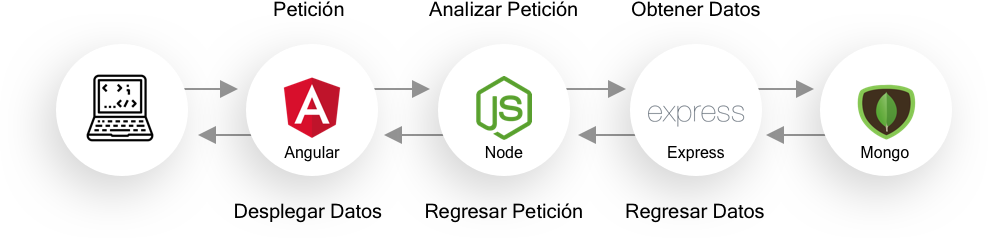
\includegraphics[width=1\textwidth]{mean}
  \caption{Flujo de información en MEAN Stack. (Fuente: Elaboración propia)}
\end{figure}

\subsection{Beneficios}
Usar JavaScript como el lenguaje de programación principal es una gran ventaja. Todo se puede configurar rápidamente y hacer en JavaScript, lo que hace que sea mucho más fácil encontrar desarrolladores, y los desarrolladores de LAMP generalmente también conocen JavaScript. Otra gran ventaja es la capacidad de crear fácilmente aplicaciones móviles o de escritorio, por ejemplo con \Gls{ionic}. El código y los componentes se pueden reutilizar o agregar fácilmente.

\subsection{Desventajas}
Muchas librerías y \glspl{framework} son bastante nuevos, y las nuevas versiones se lanzan rápidamente, por lo que mantener una aplicación puede ser una molestia. Dado que muchas tecnologías desaparecen después de unos años, la sostenibilidad puede convertirse en un problema. También es más difícil mantener una base de código limpia y seguir las mejores prácticas a medida que su aplicación crece. Además, debe confiar en el cliente y las tecnologías disponibles del cliente.

\newpage
\subsection{Base de datos NoSQL}
A pesar de la gran cantidad de bases de datos SQL, también hay una tendencia hacia NoSQL. Las bases de datos NoSQL permiten almacenar datos no estructurados y heterogéneos. La \gls{escalabilidad} mejorada ha ayudado a aumentar su popularidad en mayor medida en el mercado actual. El escalado horizontal significa que la organización no tiene que preocuparse por la infraestructura subyacente. Las bases de datos NoSQL son una alternativa emergente a las bases de datos relacionales más utilizadas. Como su nombre lo indica, no reemplaza completamente a SQL, sino que lo complementa de tal manera que puedan coexistir.
\vspace{0.8cm}

\begin{table}[H]
  \renewcommand{\arraystretch}{1.5}
  \centering
  \scriptsize
  \begin{tabular}{ |p{2cm}||p{5cm}|p{5cm}|  }
    \hline
      & SQL
      & NoSQL \\
    \hline
    Tipo
      & Relacional
      & Distribuido \\
    \hline
    Datos
      & Datos estructurados almacenados en tablas 
      & Datos no estructurados almacenados en archivos JSON \\
    \hline
    Esquema 
      & Estático o predefinido
      & Dinámico \\
    \hline
    Escalable 
      & Vertical
      & Horizontal \\
    \hline
    Consultas
      & Adecuado para consultas complejas 
      & Lenguaje de consulta no estructurado \\
    \hline
    Flexible
      & Esquema rígido ligado a la relación 
      & Esquema adecuado para almacenamiento jerárquico \\
    \hline
    Elasticidad
      & Requiere tiempo de inactividad en la mayoría de los casos 
      & Automática, no requiere interrupción \\
    \hline
  \end{tabular}
  \caption{Comparativa SQL y NoSQL}
\end{table}
\vspace{0.8cm}

El concepto de NoSQL se desarrolló hace mucho tiempo, pero fue después de la introducción de la base de datos como servicio (DBaaS) que obtuvo un reconocimiento destacado. Debido a la alta \gls{escalabilidad} proporcionada por NoSQL, fue visto como un importante competidor del modelo de base de datos relacional. A diferencia de las bases de datos relacionales (RDB), las bases de datos NoSQL están diseñadas para escalar fácilmente a medida que crecen. La mayoría de los sistemas NoSQL han eliminado el soporte multiplataforma y algunas características adicionales innecesarias de \acrshort{rdbms}, haciéndolos mucho más livianos y eficientes que sus contrapartes \acrshort{rdbms}.


\subsection{Orientado a documentos}
El concepto principal de una base de datos orientada a documentos es que el documento contiene grandes cantidades de datos que pueden estar disponibles de manera útil. Se puede acceder a estos documentos como un directorio regular en el que puede tener diferentes colecciones y cada colección tiene documentos que contienen la información deseada. Además, cada colección puede tener colecciones internas. Puede tener un árbol completo de documentos, sin embargo, esta práctica no se recomienda y debe evitar tener más de tres niveles de anidamiento. 
\vspace{0.8cm}

Las bases de datos NoSQL no son necesariamente bases de datos relacionales. Los datos no son representados en términos de filas y columnas de tablas. En MongoDB, los datos se visualizan como objetos o documentos. Esto ayuda a un programador a evitar una capa de traducción, por lo que no es necesario convertir o asignar los objetos con los que trata el código en tablas relacionales. Dichas traducciones se denominan capas de Mapeo Relacional de Objetos (ORM).
\begin{figure}[H]
  \centering
  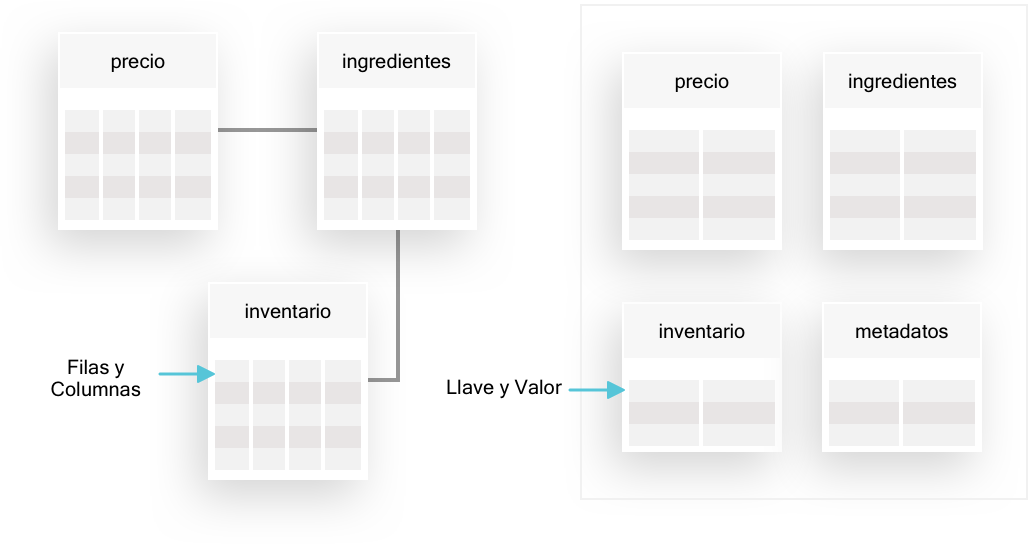
\includegraphics[width=1\textwidth]{sql-nosql}
  \caption{Diagrama que representa las diferencias clave entre la base de datos SQL y las bases de datos NoSQL. (Fuente: Elaboración propia)}
\end{figure}

\subsection{Angular/React}
Angular o React, proporcionan la interfaz de usuario reactiva de una aplicación. Utilizan componentes, son reactivos porque el usuario recibe cambios inmediatos cuando interactúa con la aplicación y, por lo general, se ejecutan dentro del navegador de un usuario (aunque ambos son \glspl{isomorfico}, capaces de ejecutarse en un servidor).
\vspace{0.8cm}

\begin{table}[H]
  \renewcommand{\arraystretch}{1.5}
  \centering
  \scriptsize
  \begin{tabular}{ |p{2cm}||p{5cm}|p{5cm}|  }
    \hline
      & Angular
      & React \\
    \hline
    Desarrollador
      & Google
      & Facebook \\
    \hline
    Definición
      & \Gls{framework}
      & Librería \\
    \hline
    Modelo de plantilla
      & HTML + Typescript
      & JSX + Javascript \\
    \hline
    Flujo
      & 2 vías
      & Unidireccional \\
    \hline
    DOM
      & Regular
      & Virtual \\
    \hline
    Lógica/Estado de la aplicación
      & Services
      & Flux/Redux \\
    \hline
  \end{tabular}
  \caption{Características de Angular.js y ReactJS}
\end{table}
\vspace{0.8cm}

Angular es un \gls{framework} con muchas herramientas integradas, para hacer solicitudes HTTP, enrutamiento y navegación, animaciones y otros. Se basa en módulos que son componentes y servicios.
\vspace{0.8cm}

React es una biblioteca de Javascript, que se puede usar para crear nuevas aplicaciones o para integrarla con una aplicación existente. React se basa en componentes pequeños y reutilizables, que administran su propio estado y luego los componen para crear interfaces de usuario complejas. Incluso si React no es tan complejo como Angular, con muchas cosas integradas, hay muchas bibliotecas que se pueden agregar para tener enrutadores (react-router) y solicitudes HTTP (\gls{axios}), manejo de estado (react-redux) entre otras más. Esto lo hace portátil y fácil de incorporar en cualquier entorno.

\newpage
\section{FERN}
Firebase es una plataforma propiedad de Google que tiene como objetivo proporcionar un enfoque completo para un rápido desarrollo web y móvil. En resumen, le permite centrarse en las partes frontales de la aplicación. Se completa con una base de datos NoSQL, alojamiento, almacenamiento de archivos, procesamiento del lado del servidor para cosas que deben protegerse de la interfaz y un sistema de autenticación, que junto a módulos de desarrollo \gls{frontend} como ReactJS, proporcionan todo lo necesario para crear aplicaciones web pequeñas y medianas.
\vspace{0.8cm}

\subsection{Componentes FERN}
\begin{itemize}
  \item Firebase (base de datos)
  \item Express.js (servidor)
  \item ReactJS (cliente)
  \item Node.js (entorno del servidor)
\end{itemize}
\begin{figure}[H]
  \centering
  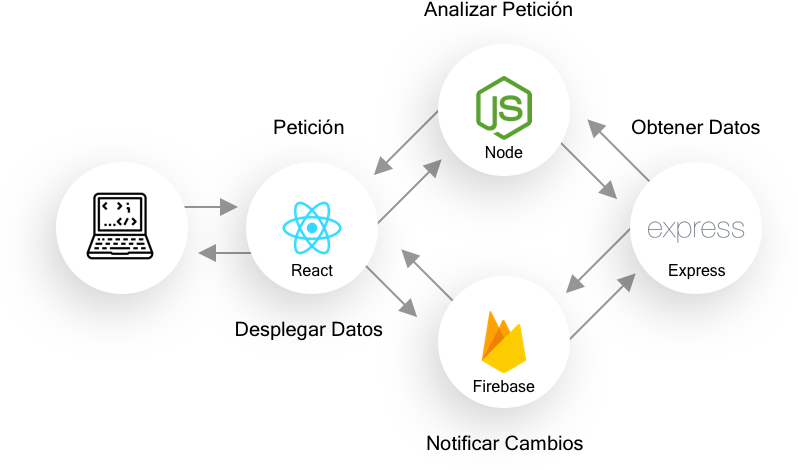
\includegraphics[width=0.8\textwidth]{fern}
  \caption{Flujo de información en FERN Stack. (Fuente: Elaboración propia)}
\end{figure}

\subsection{Cloud Firestore}
Cloud Firestore es el servicio de base de datos de Google Firebase para aplicaciones móviles. Firestore permite una experiencia de programación increíble cuando se usa en un stack de aplicaciónes completo. Los datos en tiempo real y la facilidad de conexión a la base de datos hacen que FERN Stack sea una forma rápida de conectar estas tecnologías.
\vspace{0.8cm}

Firestore es una base de datos orientada a documentos, toda la información se guarda en colecciones como en un JSON, principalmente diseñada para almacenar, recuperar y administrar información orientada a documentos, también conocida como datos semiestructurados. La \gls{escalabilidad} es completamente automática, lo que significa que no es necesario compartir sus datos en varias instancias. Los cargos de Cloud Firestore se basan en las operaciones realizadas en su base de datos (lectura, escritura, borrado), ancho de banda y almacenamiento. Admite límites de gasto diario para proyectos de Google App Engine, para garantizar que no exceda los costos con los que el usuario se sienta cómodo.
\vspace{0.8cm}

\begin{figure}[H]
  \centering
  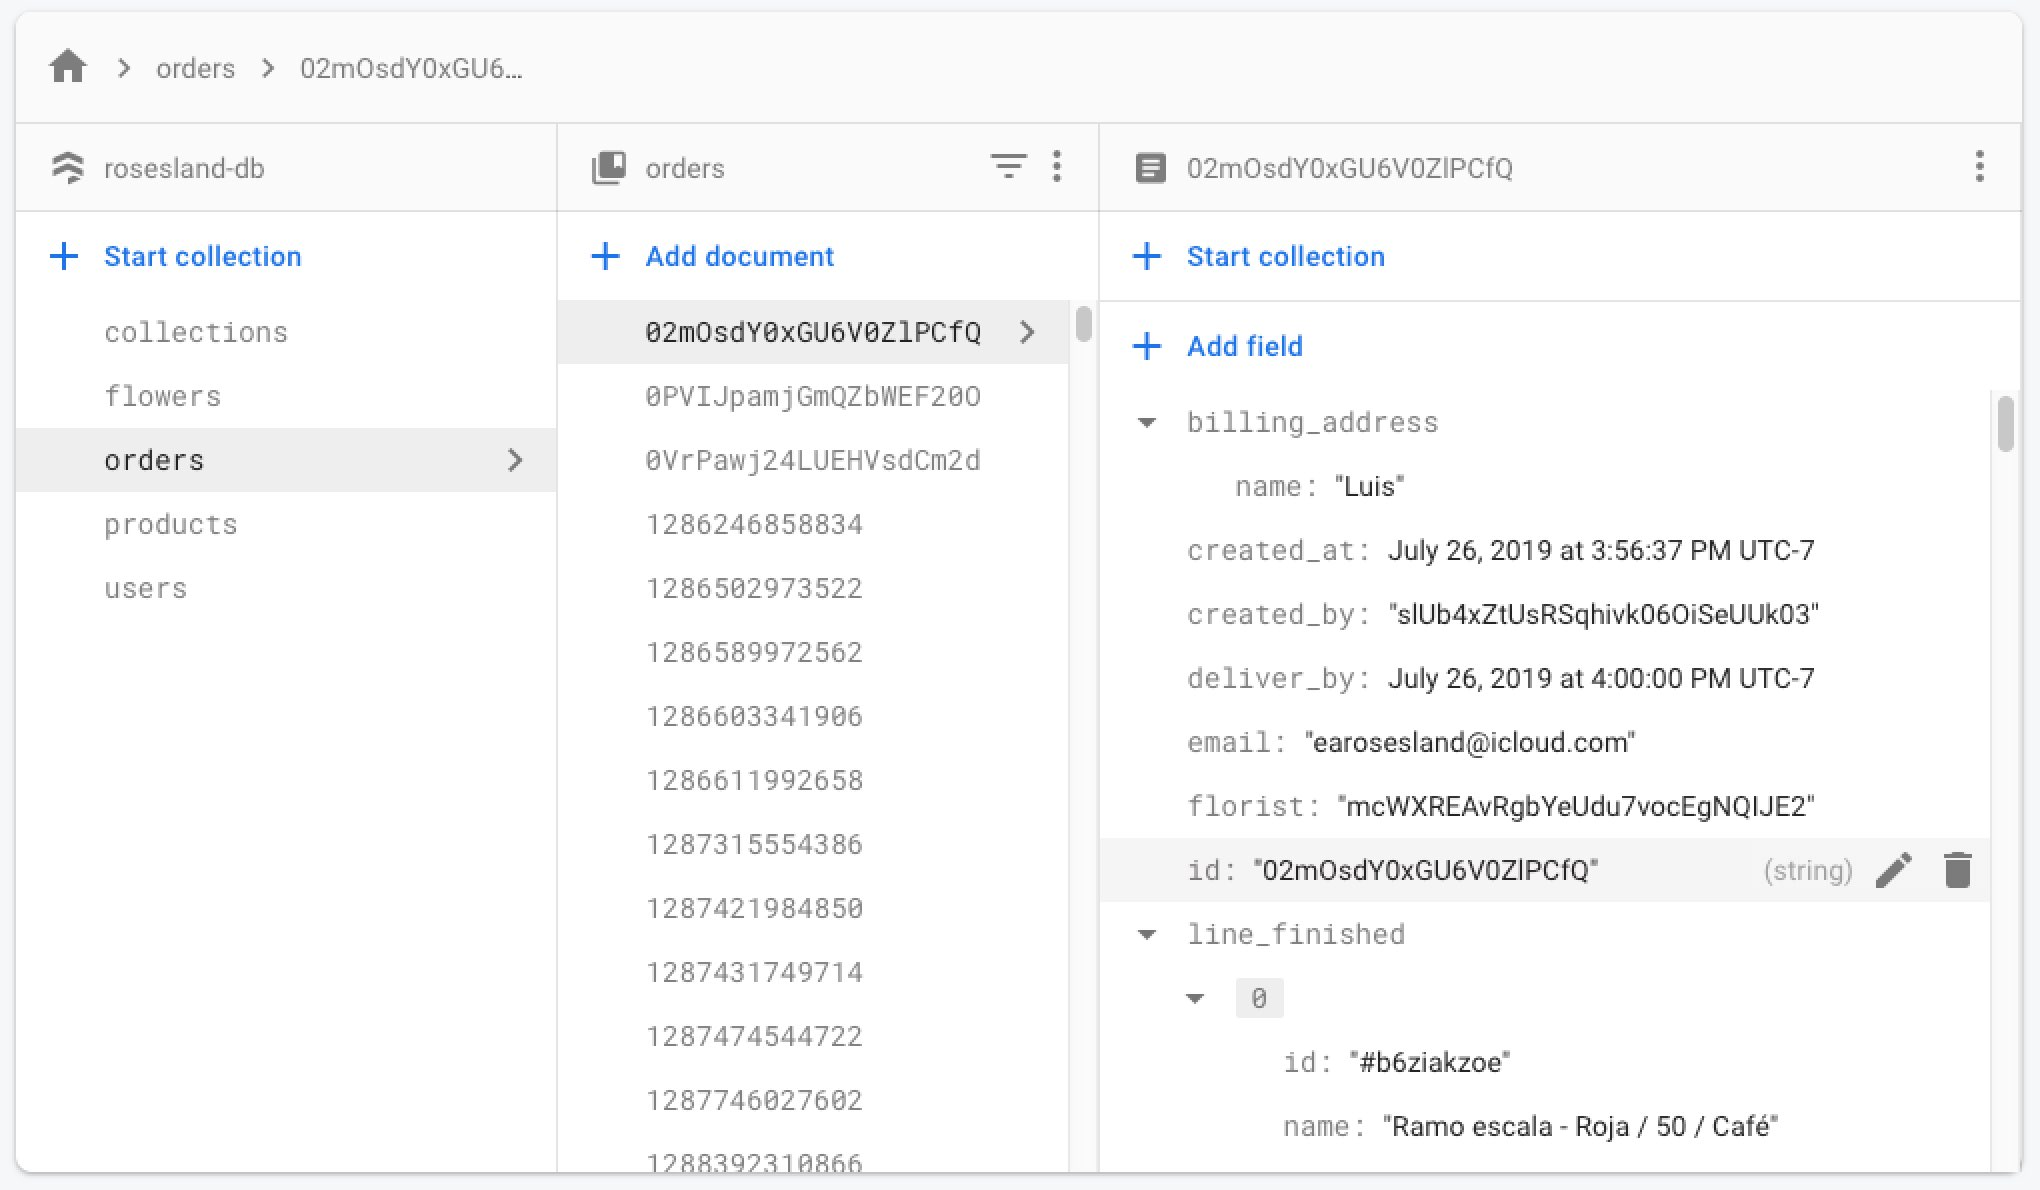
\includegraphics[width=0.9\textwidth]{firestore}
  \caption{Colección de Firestore con sus documentos internos. (Fuente: Elaboración propia)}
\end{figure}

\subsection{Node.js}
Node.js es un entorno multiplataforma de código abierto para ejecutar código JavaScript del lado del servidor. El entorno de tiempo de ejecución de Node.js incluye todo lo que necesita para ejecutar un programa escrito en JavaScript. 
\vspace{0.8cm}

Node.js surgió cuando los desarrolladores originales de JavaScript lo extendieron de algo que solo podía ejecutar en el navegador a algo que podría ejecutar en su máquina como una aplicación independiente. Ahora puede hacer mucho más con JavaScript que simplemente hacer que los sitios web sean interactivos. JavaScript ahora tiene la capacidad de hacer cosas que otros lenguajes de secuencias de comandos como Python pueden hacer. Tanto su navegador JavaScript como Node.js se ejecutan en el motor de tiempo de ejecución JavaScript V8. Este motor toma su código JavaScript y lo convierte en un código de máquina más rápido. El código de máquina es un código de bajo nivel que la computadora puede ejecutar sin necesidad de interpretarlo primero.
\vspace{0.8cm}

\begin{figure}[H]
  \centering
  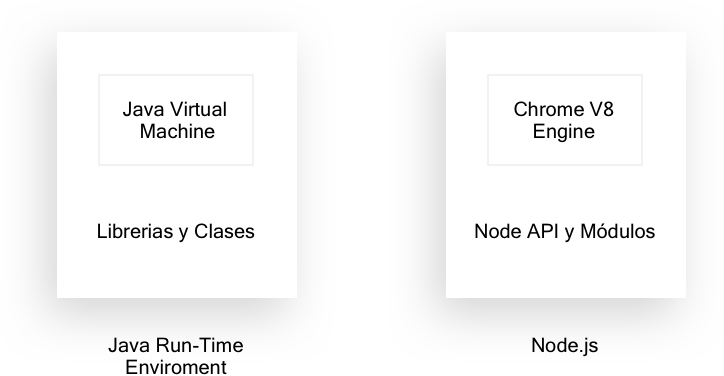
\includegraphics[width=0.8\textwidth]{node}
  \caption{Analogía Node.js con Java. (Fuente: Elaboración propia)}
\end{figure}
% \vspace{0.8cm}

\subsubsection{Motor V8 de Google Chrome}
Node.js utiliza el motor de ejecución ultra rápido V8 de Google Chrome. Hasta el lanzamiento de Chrome, la mayoría de los navegadores leían JavaScript de manera ineficiente: el código se leía e interpretaba poco a poco. Tomó mucho tiempo leer JavaScript y convertirlo a lenguaje máquina para que el procesador pudiera entenderlo. 
\vspace{0.8cm}

El motor V8 de Google Chrome funciona completamente diferente. Está altamente optimizado y lleva a cabo lo que llamamos compilación \acrshort{jit} (Just In Time). Transforma rápidamente el código JavaScript en lenguaje máquina.
\vspace{0.8cm}

\begin{table}[H]
  \renewcommand{\arraystretch}{1.5}
  \centering
  \scriptsize
  \begin{tabular}{ |p{2cm}||p{5cm}|p{5cm}|  }
    \hline
        Navegador
      & Motor de \gls{renderizado} / diseño
      & Motor de secuencias de comandos \\
    \hline
        Chrome
      & Blink (C++)
      & V8 (C++) \\
    \hline
    \hline
        Mozilla Firefox
      & Gecko (C++)
      & SpiderMonkey (C/C++) \\
    \hline
    \hline
        IE Edge
      & EdgeHTML (C++)
      & Chakra JavaScript engine (C++) \\
    \hline
    \hline
    Opera
      & Blink (C++)
      & V8 (C++) \\
    \hline
    Internet Explorer
      & Trident (C++)
      & Chakra JScript engine (C++) \\
    \hline
  \end{tabular}
  \caption{Motores de renderizado y secuencias de comandos}
\end{table}
\vspace{0.8cm}


\subsection{El ecosistema NPM}
NPM (Node Package Manager) es el administrador de paquetes predeterminado para Node.js. Paquete es un término utilizado por npm para denotar herramientas que los desarrolladores pueden usar para sus proyectos \cite{goalkicker-node}. Se instala en el sistema con la instalación de Node.js. Los paquetes y módulos necesarios en un proyecto Node se instalan utilizando \textit{npm}.
\vspace{0.8cm}

NPM consta de tres componentes:
\begin{enumerate}
  \item Sitio web
  \item Registro
  \item CLI
\end{enumerate}
\subsubsection{Sitio web}
El sitio web oficial de npm es https://www.npmjs.com/. Con este sitio web puede encontrar paquetes, ver documentación, compartir y publicar paquetes.
\subsubsection{Registro}
El registro npm es una gran base de datos que consta de más de medio millón de paquetes. Los desarrolladores descargan paquetes del registro npm y publican sus paquetes en el registro.
\subsubsection{CLI (interfaz de línea de comando)}
Esta es la línea de comando que ayuda a interactuar con el npm para instalar, actualizar y desinstalar paquetes y administrar dependencias.
\subsection{Comandos NPM}
Npm tiene muchos paquetes que puedes usar en una aplicación para que su desarrollo sea más rápido y eficiente. Instalar módulos usando NPM no representa un gran problema. Hay una sintaxis simple para instalar cualquier módulo Node.js:
\vspace{0.8cm}

% \begin{verbatim}
%   npm install nombre-del-paquete
%   ejemplo: npm install express
% \end{verbatim}
\begin{lstlisting}[language=HTML]
  npm install nombre-del-paquete
  ejemplo: npm install express
\end{lstlisting}
% \lstinputlisting[style=ES6, caption=Comandos para instalar paquete con NPM]{code/npm.txt}

\subsection{Express.js}
Escribir un servidor web completo a mano en Node.js directamente no es tan fácil, ni es necesario, Express.js es un paquete de aplicación web minimalista y extensible creado para el ecosistema Node.js. Permite crear un servidor web legible, flexible y fácil de mantener.
\vspace{0.8cm}

Express.js le permite definir rutas, especificaciones de qué hacer cuando llega una solicitud HTTP que coincide con un patrón determinado. La especificación coincidente se basa en expresiones regulares (regex) y es muy flexible, como la mayoría de los otros entornos de aplicaciones web. La parte de qué hacer es solo una función que recibe la solicitud HTTP analizada.
\vspace{0.8cm}

Express.js analiza la URL de solicitud, encabezados y parámetros. En el lado de la respuesta, tiene, como se esperaba, toda la funcionalidad requerida por las aplicaciones web. Esto incluye la configuración de códigos de respuesta, configuración de \glspl{cookie}, envío de encabezados personalizados, etc. Además, puede escribir middleware Express, piezas de código personalizadas que se pueden insertar en cualquier ruta de procesamiento de solicitud/respuesta para lograr una funcionalidad común como el registro, la autenticación, entre otras.
\vspace{0.8cm}


\lstinputlisting[style=ES6, caption=Simple aplicación Express.js]{code/express.js}

\subsection{ReactJS}
React es una biblioteca de JavaScript declarativa, eficiente y flexible creada en 2013 por el equipo de desarrollo de Facebook. React quería que las interfaces de usuario fueran más modulares (o reutilizables) y más fáciles de mantener. Según el sitio web de React, se utiliza para \textit{construir componentes encapsulados que administran su propio estado, y unirlos para crear interfaces de usuario complejas}. React es una biblioteca JavaScript que permite componer interfaces de usuario complejas a partir de piezas de código pequeñas y aisladas llamadas \textit{componentes}.
\vspace{0.8cm}

En términos generales, al crear aplicaciones con ReactJS, se crean componentes que corresponden a distintos elementos de una interfaz de usuario. Después se organizan estos elementos dentro de componentes de orden superior que definen la estructura de la aplicación. Es importante destacar que cada componente en una aplicación React se rige por principios estrictos de gestión de datos. Interfaces avanzadas comúnmente involucran datos complejos y manejo de estado. ReactJS es limitado y tiene como objetivo darnos las herramientas para poder anticipar cómo se verá una aplicación con un conjunto de circunstancias dado.

\subsection{Componentes React}
Un componente es una pequeña parte de la interfaz de usuario. Todas las piezas reutilizables de una página web se abstraen en estos elementos. Son similares, en conceptos, a cosas como \glspl{widget} y módulos. React se define a sí mismo como una biblioteca para construir interfaces de usuario. Como tal, cuando se piensa en una interfaz de usuario, se debe pensar en ella en términos de los componentes más pequeños posibles que se puedan definir. La razón por la que existe este paradigma es para disminuir el acoplamiento (cuánto dependen los unos de los otros) y aumentar la cohesión (qué tan bien funcionan juntas las diferentes cosas).
\vspace{0.8cm}

Cada uno de estos fragmentos es un bloque de código independiente y reutilizable, que divide la interfaz de usuario en partes más pequeñas. Incluyen código que define cómo se crean los elementos en el \acrshort{dom} y cómo los usuarios pueden interactuar con ellos. Los componentes se pueden definir únicamente en JavaScript o se pueden definir en un superconjunto (o variación extendida) de JavaScript llamado JSX, que se explica en temas posteriores.
\vspace{0.8cm}

\begin{figure}[H]
  \centering
  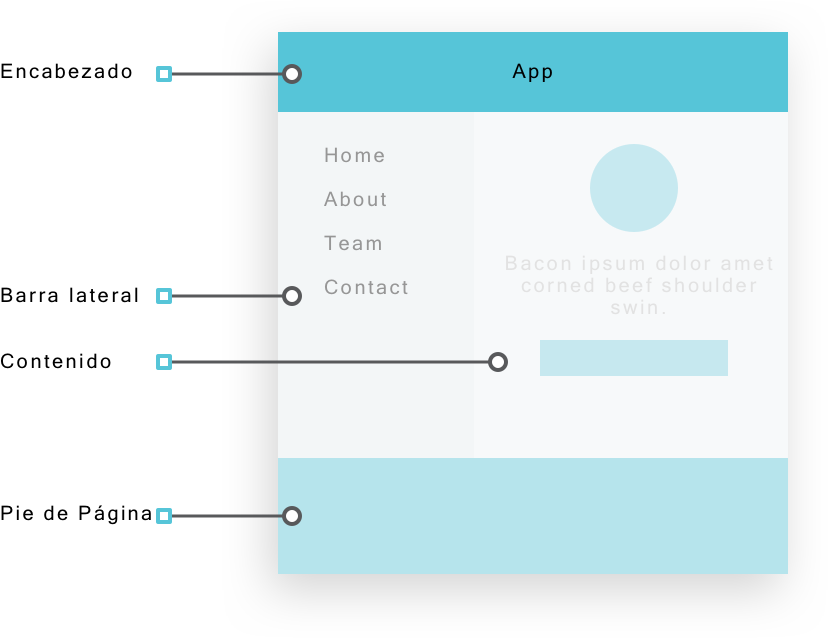
\includegraphics[width=0.8\textwidth]{components}
  \caption{Componentes principales de una página web. (Fuente: Elaboración propia)}
\end{figure}
En primer lugar, hay un elemento principal llamado componente APP. Este componente de la aplicación contiene cuatro fragmentos secundarios o se divide en cuatro componentes:
\begin{enumerate}
  \item Encabezado
  \item Barra lateral
  \item Contenido
  \item Pie de página
\end{enumerate}
La función de cada componente se manejará independientemente con otros componentes. Cada componente es una pieza reutilizable, y se puede pensar en cada componente de forma aislada.
\vspace{0.8cm}

Dentro de un componente, tendremos subcomponentes o componentes dentro de un componente padre. Esos serán reutilizables también. En pocas palabras, un componente es una clase o función de JavaScript que opcionalmente acepta entradas, es decir, propiedades (props) y devuelve un elemento que describe cómo debería lucir una sección de la interfaz de usuario.
\vspace{0.8cm}

\lstinputlisting[style=ES6, caption=Ejemplo de página con componentes ReactJS]{code/react-example.js}

\subsection{DOM Virtual}
En el desarrollo web de software, \acrshort{dom} significa Modelo de Objeto de Documento (Document Object Model) y representa la estructura de los elementos en una página web. El HTML DOM se construye como un árbol de objetos.

Algunas bibliotecas de JavaScript, como jQuery, manipulan los elementos DOM directamente, cambiando sus atributos, agregando o eliminando componentes. Sin embargo, en lugar de cambiar el DOM directamente, React usa un DOM virtual, que es una replicación virtual del árbol DOM actual. En consecuencia, React puede manipular el DOM virtual innumerables veces y comparar su estado con el DOM real. De esta manera, React sabe exactamente qué elemento cambió y luego actualiza solo ese elemento específico en la pantalla.

Detrás de escena, React hace un gran trabajo para editar y volver a \gls{renderizar} eficientemente el DOM cuando algo en la interfaz necesita cambiar. Este enfoque le brinda al desarrollador una gran flexibilidad y sorprendentes ganancias de rendimiento porque ReactJS calcula con anticipación qué cambios se deben realizar en el DOM y actualiza los árboles DOM en consecuencia. De esta manera, ReactJS evita las costosas operaciones DOM y realiza actualizaciones de manera eficiente \cite{stefanov}.


\newpage
\section{Preprocesamiento}
\subsection{ES5/ES6}
ES5 (ES significa ECMAScript) es básicamente `JavaScript normal'. La quinta actualización de JavaScript, ES5 se finalizó en 2009. Ha sido compatible con todos los principales navegadores durante muchos años. \\[0.8cm]
ES6 es una nueva versión de JavaScript que agrega algunas buenas adiciones sintácticas y funcionales. Se finalizó en 2015. ES6 es casi totalmente compatible con todos los navegadores principales. Pero pasará algún tiempo hasta que las versiones anteriores de los navegadores web estén fuera de uso. Por ejemplo, Internet Eyplorer 11 no es compatible con ES6, pero tiene aproximadamente el 8\% de uso de mercado de navegadores.\\[0.8cm]
Para aprovechar los beneficios de ES6 hoy, se tienen que hacer que hacer algunos procedimientos para que funcione en tantos exploradores de internet como sea posible:
\begin{enumerate}
  \item Se debe preprocesar el código para que una gama más amplia de navegadores entiendan nuestro JavaScript. Esto significa convertir ES6 JavaScript en ES5 JavaScript.
  \item Tenemos que incluir un `shim' o `polyfill' que brinde una funcionalidad adicional agregada en ES6 que un navegador puede o no tener.
\end{enumerate}
\subsubsection{JSX}
JSX es una extensión de sintaxis similar a XML para ECMAScript sin ninguna semántica definida. NO está destinado a ser implementado por motores o navegadores. NO es una propuesta para incorporar JSX en la propia especificación ECMAScript. Está destinado a ser utilizado por varios preprocesadores (transpiladores) para transformar estos \glspl{token} en ECMAScript estándar.
\subsubsection{BabelJS}
BabelJS es un transpilador de JavaScript que transpila nuevas características ES6 al antiguo estándar ES5. Con esto, las funciones se pueden ejecutar en navegadores antiguos y nuevos, sin problemas. \\[0.8cm]
\textbf{El preprocesador BabelJS} convierte la sintaxis de JavaScript moderno en un formulario, que los navegadores más antiguos pueden entender fácilmente. Por ejemplo, const y let se convertirán en var, la función flecha se convierte en una función normal manteniendo la funcionalidad igual en ambos casos. \\[0.8cm]

\lstinputlisting[style=ES6, caption=Ejemplo de sintaxis ES5 y ES6]{code/es5-es6.js}

\subsubsection{Sass (Syntactically Awesome Style Sheets)}
Sass es un preprocesador de CSS, que ayuda a reducir la repetición con CSS y ahorra tiempo. Es un lenguaje de extensión CSS más estable y potente que describe el estilo de una página estructuralmente. Sus principales atributos son:
\begin{enumerate}
  \item Es un súper conjunto de CSS, lo que significa que contiene todas las características de CSS y es un preprocesador de código abierto, codificado en Ruby.
  \item Proporciona algunas características, que se utilizan para crear hojas de estilo que permiten escribir código más eficiente y fácil de mantener.
\end{enumerate}
\subsubsection{Webpack}
Webpack es un empaquetador de módulos. Webpack toma un archivo de entrada, encuentra todos los archivos de los que depende y genera un archivo que contiene todo el código de una aplicación. Con él es posible importar archivos CSS e imágenes directamente a JavaScript. Se puede compilar CoffeeScript, TypeScript, SASS y LESS. También es capaz de compilar la sintaxis de ES6 en JavaScript amigable para el navegador. En otras palabras, Webpack toma diferentes archivos (como CSS, JS, SASS, JPG, SVG, PNG, etc.) y los combina en paquetes, un paquete separado para cada tipo de archivo.


% \begin{lstlisting}[style=ES6, caption=Ejemplo de sintaxis ES5 y ES6]
%   // Extraer de objetos

%   var obj1 = { a: 1, b: 2 };
% \end{lstlisting}

\newpage
\section{Control de versiones}
Hoy en día no es prudente empezar un proyecto web sin una estrategia de respaldo. Debido a que los datos son efímeros y se pueden perder fácilmente, por ejemplo, a través de un cambio de código erróneo o un fallo catastrófico de disco, es aconsejable mantener un archivo de todo el trabajo.\\[0.8cm]
Para proyectos de texto y código, la estrategia de respaldo generalmente incluye control de versiones, o seguimiento y administración de revisiones.  Dado su papel fundamental, el control de versiones es más efectivo cuando se adapta a los hábitos y objetivos de trabajo del equipo del proyecto.\\[0.8cm]
En su forma más simple, un sistema de control de versiones proporciona un principio básico y un método para almacenar archivos y cambios realizados en ellos. Esto se logra mediante el uso de un repositorio. El repositorio contiene la versión más reciente de cada archivo y el historial de cambios que ha llevado a esa representación. Por lo general, cada cambio incluye información adicional, como el autor y una breve descripción.
\subsection{Git}
Git es un software de control de versiones distribuido particularmente potente, flexible y de bajo costo que hace que el desarrollo colaborativo sea un placer. \\[0.8cm]
La principal diferencia entre Git y cualquier otro versionador es la forma en que Git piensa acerca de sus datos. Conceptualmente, la mayoría de los otros sistemas almacenan información como una lista de cambios basados en archivos. Estos sistemas (CVS, Subversion, Perforce, Bazaar, etc.) piensan en la información que mantienen como un conjunto de archivos y los cambios realizados en cada archivo a lo largo del tiempo. Git no piensa ni almacena sus datos de esta manera. En cambio, Git piensa en sus datos más como un conjunto de instantáneas de un mini sistema de archivos. Cada vez que confirma o guarda el estado de su proyecto en Git, básicamente toma una fotografía de cómo se ven todos sus archivos en ese momento y almacena una referencia a esa instantánea. Para ser eficiente, si los archivos no han cambiado, Git no almacena el archivo nuevamente, solo un enlace al archivo idéntico anterior que ya ha almacenado. \\[0.8cm]
\begin{figure}[H]
  \centering
  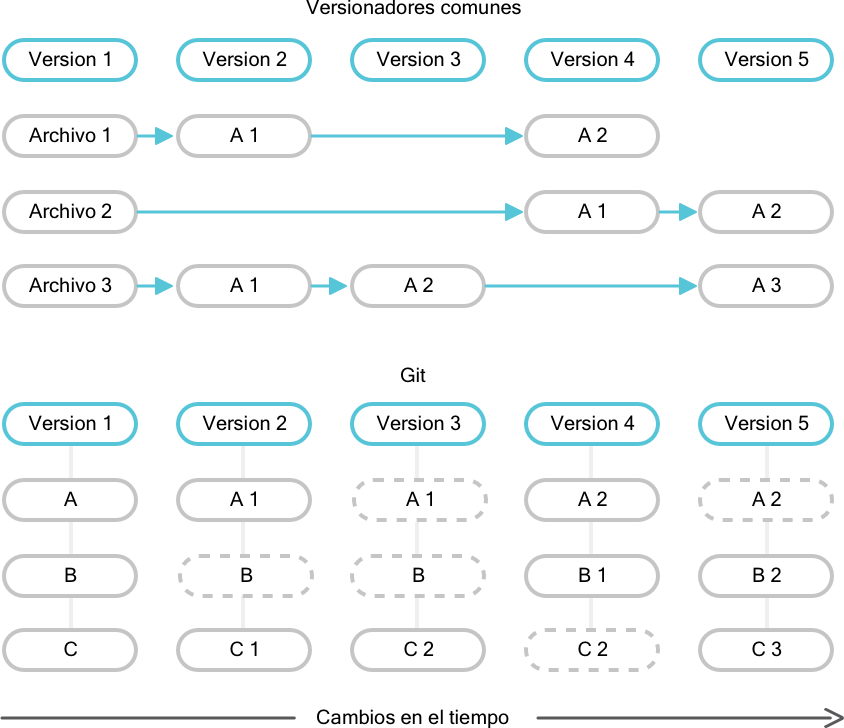
\includegraphics[width=0.9\textwidth]{git}
  \caption{Diferencias entre controladores de versiones. (Fuente: Elaboración propia)}
\end{figure}

\chapter{Análisis y diseño del sistema}
A continuación se describen los procedimientos necesarios para elaborar un sistema que permita elaborar y mostrar sugerencias de caminabilidad en el área de tijuana, así como incorporar servicios de geolocalización..

\section{Requerimientos del proyecto}
El sistema debe adaptarse al sistema operativo Linux. Anticipado a futuros cambios en la plataforma se decide trabajar con Node.js, ya que es de código abierto y multiplataforma, esto permite beneficiarse de la reutilización del código y la falta de cambio de contexto. Las aplicaciones Node.js están escritas en JavaScript puro y pueden ejecutarse dentro del entorno Node.js en Windows, Linux, etc.
\vspace{0.8cm}

La interfaz gráfica de usuario de la aplicación debe ser responsiva y funcionar en la mayoría de los navegadores web modernos, además debe ser fácil de aprender, idealmente requerir poco entrenamiento.
\vspace{0.8cm}

\subsection{Herramientas}
Node.js permite incorporar herramientas poderosas a proyectos de cualquier tipo. Esto incluye todo, desde bibliotecas y \glspl{framework} como jQuery y AngularJS hasta procesadores de código como Webpack. Los paquetes vendrán en una carpeta típicamente llamada node\_modules, que también contendrá un archivo package.json. Este archivo contiene información sobre todos los paquetes, incluidas las dependencias, que son módulos adicionales necesarios para usar un paquete en particular.

\subsubsection{Dependencias de desarrollo}
Las dependencias de desarrollo son aquellas que se utilizan dentro del entorno de programación. Aquí se incluyen herramientas que no forman parte del ejecutable final como lo son lo preprocesadores, empaquetadores y analistas de código. Los principales módulos de desarrollo son los siguientes:
\begin{itemize}
  \item Babel: es un compilador de JavaScript utilizado para convertir código ECMAScript 2015+ (ES6+) en una versión que pueda ser ejecutado en motores JavaScript más antiguos.
  \item Webpack: es un empaquetador de módulos principalmente para JavaScript, pero puede transformar archivos \gls{frontend} como HTML, CSS e imágenes si se incluyen los complementos correspondientes.
  \item ESLint: es una herramienta de análisis de código estático para identificar patrones problemáticos encontrados en el código JavaScript.
  \item PostCSS: es una herramienta de desarrollo de software que utiliza complementos basados en JavaScript para automatizar las operaciones de rutina de CSS. Con este modulo es posible analizar CSS, agregar prefijos de proveedor a las reglas CSS, ejecutar optimizaciones enfocadas, para garantizar que el resultado final sea lo más pequeño posible para un entorno de producción.
  \item Pug: es un preprocesador que simplifica la tarea de escribir HTML. También agrega funcionalidades, como objetos Javascript, condiciones, bucles, \glspl{mixin} y plantillas.
\end{itemize}

\subsubsection{Estructura del proyecto}
La estructura del proyecto Node.js está influenciada por preferencias personales, la arquitectura del proyecto y la estrategia de inyección de módulos que se está utilizando. Para tener una estructura FERN, es imperativo separar el código fuente del servidor y el utilizado por el cliente, ya que el código del lado del cliente o \gls{frontend} probablemente se minimizará y se enviará al navegador y es público en su naturaleza básica. Y el lado del servidor o el \gls{backend} proporcionarán \acrshort{api} para realizar operaciones \acrshort{crud}.

\subsubsection{Directorios}
\begin{itemize}
  \item node\_modules: Directorio oculto que contiene las dependencias generales del proyecto, este archivo debe ser ignorado por el controlador de versiones.
  \item server: Aquí se encuentran los archivos requeridos por el servidor para el enrutamiento, la conexión con la base de datos y las funciones de utilidad del \gls{backend}.
  \item src: Este directorio concentra todos los elementos necesarios para producir nuestra aplicación cliente.
  \item views: En esta carpeta se incluyen los templates necesarios para generar las vistas HTML de nuestro proyecto.
  \item www: Su propósito es contener los archivos del cliente, aquí podemos encontrar el código de producción de nuestra aplicación web compilado y minificado, así como las hojas de estilo, imágenes, fuentes tipográficas, vectores, etc.
\end{itemize}

\subsubsection{Archivos principales}
\begin{itemize}
  \item .babelrc: Contiene los mecanismos necesarios para compilar sintaxis moderna de JavaScript y una lista con los navegadores web a los que se requiere dar enfoque.
  \item .env: Documento oculto que contiene las variables del entorno, este archivo es ignorado por el controlador de versiones.
  \item .eslintrc.js: En este archivo se declaran las reglas para identificar e informar sobre patrones o errores encontrados en el código.
  \item .gitignore: Aquí se describen los archivos y directorios que deben ser ignorados por Git.
  \item index.js: Entrada principal de nuestro servidor, contiene el código necesario para que el proyecto funcione correctamente.
  \item package.json: Este archivo puede contener muchos metadatos sobre su proyecto. Pero principalmente se usa para dos cosas:
  \begin{itemize}
    \item Gestionar dependencias de su proyecto
    \item Scripts, que ayudan a generar compilaciones, ejecutar pruebas y otras cosas con respecto al proyecto
  \end{itemize}
\end{itemize}

\begin{figure}[H]
  \centering
  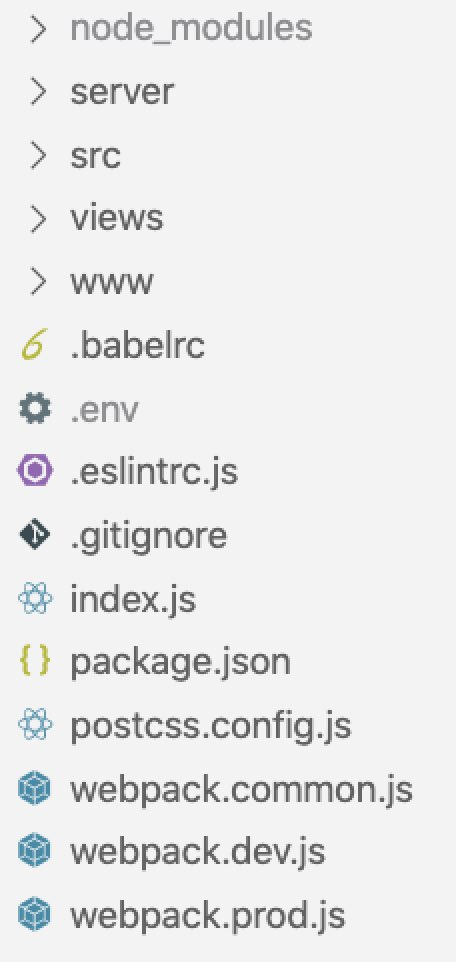
\includegraphics[width=0.3\textwidth]{app}
  \caption{Vista general de la raíz del proyecto. (Fuente: Elaboración propia)}
\end{figure}

\newpage
\subsubsection{Variables del entorno}
El acceso a las variables de entorno en Node.js es compatible desde el primer momento. Cuando el proceso Node.js se inicia, automáticamente proporciona acceso a todas las variables de entorno existentes al crear un objeto env como propiedad del objeto global del proceso.
\vspace{0.8cm}

\lstinputlisting[style=ES6, caption=Variables principales del sistema]{code/env.txt}


\newpage
\section{Configuración del servidor (Backend)}
Si alguna vez ha utilizado PHP o ASP, probablemente esté acostumbrado a la idea de que el servidor web (Apache o IIS, por ejemplo) sirve sus archivos estáticos para que un navegador puede verlos a través de la red. Node ofrece un paradigma diferente al de un servidor web tradicional: la aplicación es el servidor web. Node simplemente proporciona las bases para que se pueda construir un servidor web. 

\subsection{Servidor NodeJS}
El modelo de E/S impulsado por eventos sin bloqueo le brinda a NodeJS un rendimiento muy atractivo, superando fácilmente los entornos de servidores como PHP y Ruby on Rails, que bloquean las E/S y manejan múltiples usuarios simultáneos en hilos separados para cada uno. Algo importante que se debe saber es que NodeJS no es un \gls{framework} sino un entorno, hay \glspl{framework} que funcionan con Node, como Express y Sails, lo que facilita la creación de aplicaciones.
\vspace{0.8cm}

\begin{figure}[H]
  \centering
  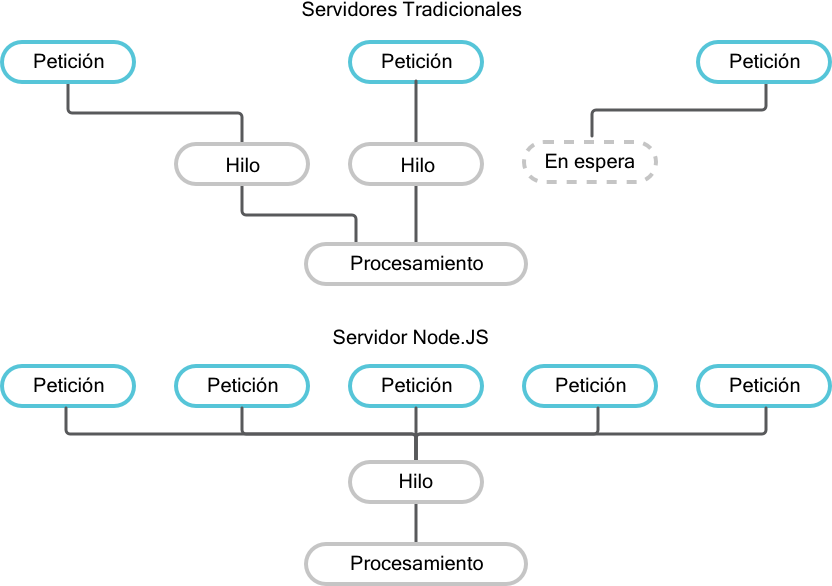
\includegraphics[width=0.8\textwidth]{node-traditional}
  \caption{Comparación de node y servidores tradicionales. (Fuente: Advance Idea Infotech 2018)}
\end{figure}

Un servidor Node.js tiene un solo subproceso de bucle de eventos (event-loop) que espera E/S en sockets y archivos. Una vez que los datos están listos, activa el método de evento correspondiente y espera hasta que regrese antes de esperar nuevamente por más eventos de E/S. Dado que todas las operaciones de E/S no bloquean, se asegurará de que todo se ejecute correctamente tan pronto como la entrada esté disponible sin ningún bloqueo y sin que se tenga lidiar con problemas de subprocesos múltiples.

\newpage
\subsubsection{Programación basada en eventos}
La filosofía central detrás de NodeJS es la programación basada en eventos. Significa que, el programador,  debe comprender qué eventos están disponibles y cómo responder a ellos. Muchas personas se introducen en la programación basada en eventos mediante la implementación de una interfaz de usuario: el usuario hace clic en algo y se dispara el `evento clic'. Es una buena metáfora, porque se entiende que el programador no tiene control sobre cuándo, o si el usuario va a hacer clic en algo, por lo que la programación basada en eventos es realmente bastante intuitiva \cite{ethan}.
\vspace{0.8cm}

\lstinputlisting[label={node-server}, style=ES6, caption=Configuración servidor NodeJS básico]{code/node-server.js}
En el ejemplo de código \ref{node-server}, el evento es implícito: el evento que se está manejando es una solicitud HTTP. El método http.createServer toma una función como argumento; esta función se invocará cada vez que se realice una solicitud HTTP. El programa simplemente establece el tipo de contenido en texto sin formato y envía la cadena `Hola, mundo!'.


\subsection{Configuración Express}
Express.js es un `marco de aplicación web NodeJS minimalista y flexible' \cite{express}. Es una capa delgada de características, fundamental para cualquier aplicación web, agrega tres características poderosas: enrutamiento, mejores manejadores de solicitudes y vistas.

\subsubsection{Enrutamiento}
Enrutamiento se refiere al mecanismo para servir al cliente el contenido que ha solicitado. Para las aplicaciones cliente/servidor basadas en web, el cliente especifica el contenido deseado en la URL (ruta y cadena de consulta).\\[0.8cm]
Cuando una aplicación Express.js se está ejecutando, escucha las solicitudes. Cada solicitud entrante se procesa de acuerdo con una cadena definida de middlewares y rutas que comienzan de arriba a abajo. Este aspecto es importante porque le permite controlar el flujo de ejecución \cite{azat}.
\vspace{0.8cm}

\begin{figure}[H]
  \centering
  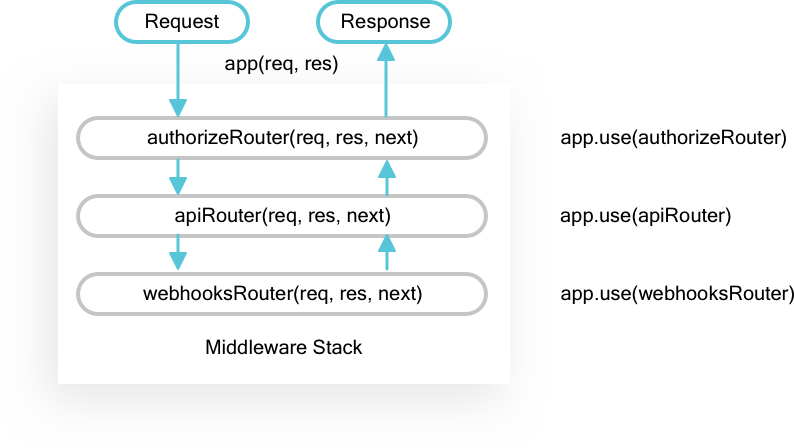
\includegraphics[width=0.8\textwidth]{express-router}
  \caption{Cada función de middleware en la pila se ejecuta antes que las que están debajo de ella. (Fuente: Elaboración propia)}
\end{figure}

\newpage
\lstinputlisting[style=ES6, caption=Fragmento de la configuración de enrutamiento del sistema]{code/express-router.js}

\subsection{Configuración Firebase}
Antes de conectar nuestro sistema con una base de datos de Firestore es necesario crear una aplicación en la consola de Google Firebase y seguir los siguientes pasos.
\vspace{0.8cm}

\begin{figure}[H]
  \centering
  
\includegraphics[width=1\textwidth]{firebase-01}
  \caption{Consola de Google Firebase. (Fuente: Google Console)}
\end{figure}

\begin{enumerate}
  \item Crear un nuevo proyecto en la consola de Firebase.

  \begin{figure}[H]
    \centering
    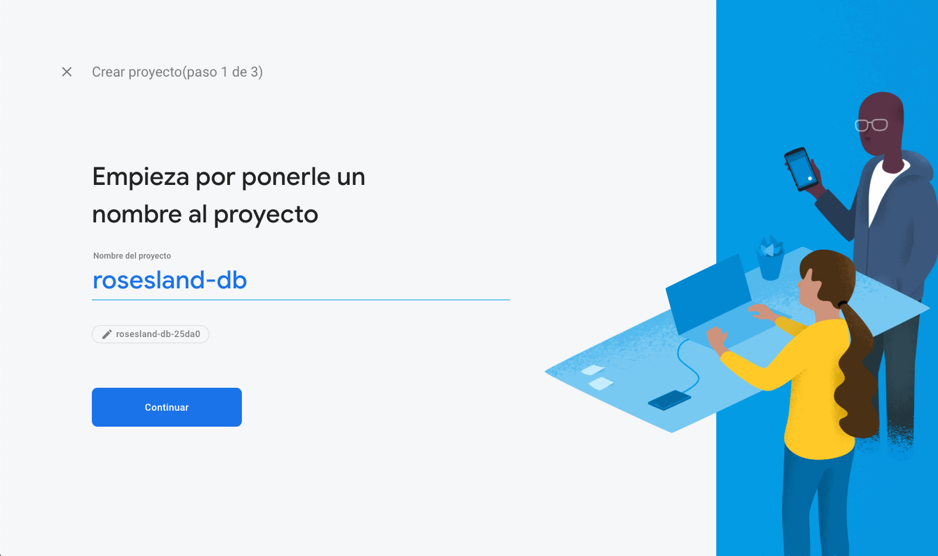
\includegraphics[width=1\textwidth]{firebase-02}
  \end{figure}

  \item En el apartado `Database', seleccionar `crear base de datos' .

  \begin{figure}[H]
    \centering
    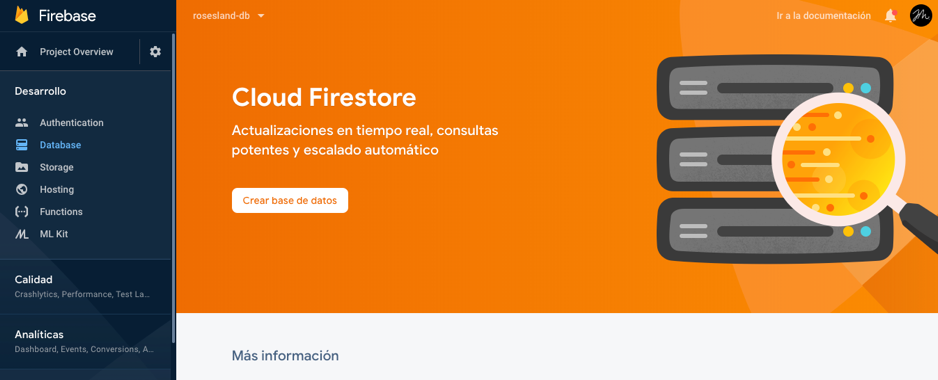
\includegraphics[width=1\textwidth]{firebase-03}
  \end{figure}

  \item En la ventana emergente, seleccionar reglas de seguridad y definir ubicación del servidor.

  \begin{figure}[H]
    \centering
    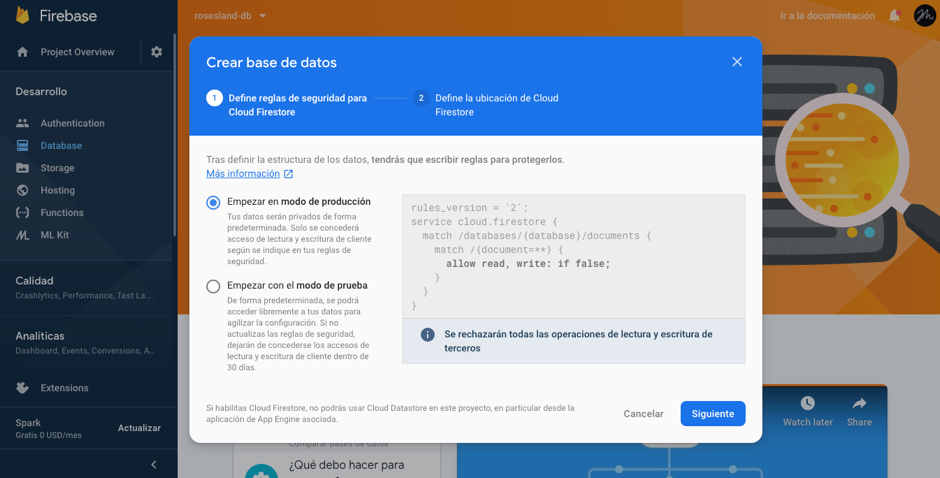
\includegraphics[width=1\textwidth]{firebase-04}
  \end{figure}

  \item El siguiente paso es generar las claves que permitan usar `firebase-admin' en el \gls{backend}. En la configuración del proyecto debajo del apartado `cuentas de servicio', presionar el botón `Generar cuentas de servicio'. El contenido del archivo JSON generado se debe de agregar a las variables del entorno que correspondan.

  \begin{figure}[H]
    \centering
    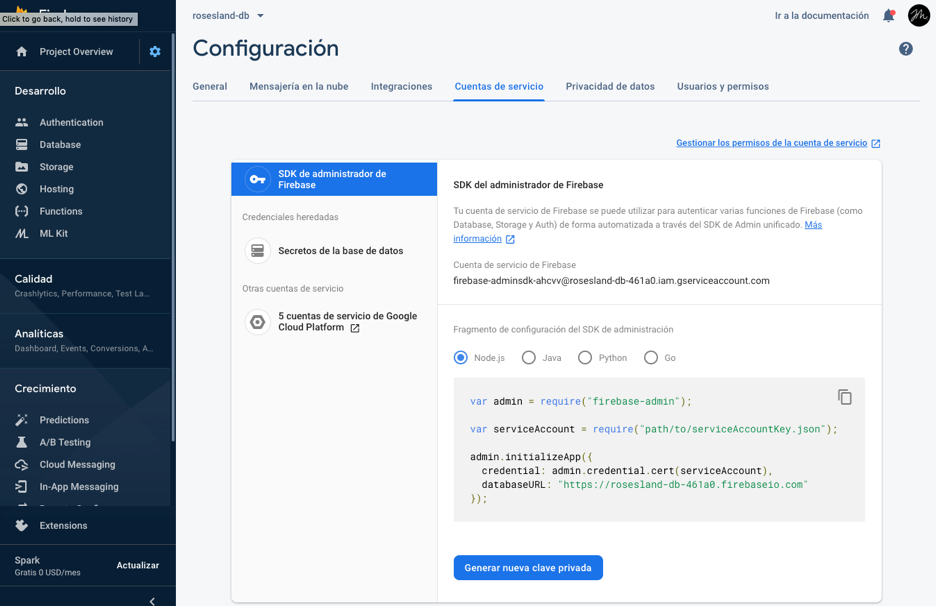
\includegraphics[width=1\textwidth]{firebase-05}
  \end{figure}

  \item Por ultimo en la sección `Authentication' se deben activar los servicios de autenticación necesarios, para este proyecto es necesario activar la validación por correo electrónico y contraseña.

  \begin{figure}[H]
    \centering
    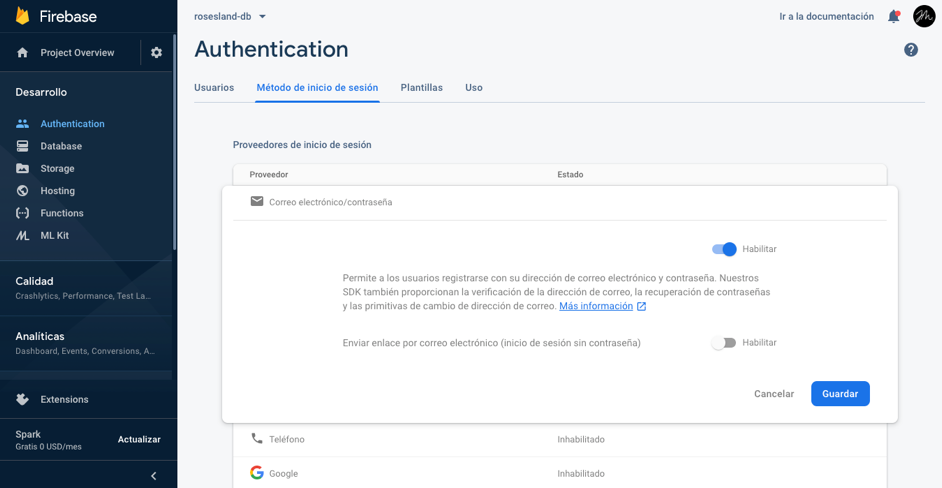
\includegraphics[width=1\textwidth]{firebase-06}
  \end{figure}
\end{enumerate}

\newpage
\subsubsection{Configuración de Firebase Firestore en Node.js}
Después de crear el objeto de configuración, es necesario inicializar Firebase en la aplicación de la siguiente manera:
\vspace{0.8cm}

\lstinputlisting[label={node-firebase}, style=ES6, caption=Fragmento de la configuración Firebase en el servidor]{code/firebase.js}

\subsubsection{Escrituras en lotes}
Para manipular documentos en un conjunto de operaciones, se pueden ejecutar varias operaciones de escritura como un lote único que incluya cualquier combinación de operaciones set(), update() o delete(). El lote de escrituras se completa de forma atómica y puede escribir en varios documentos. Los siguientes ejemplos muestran cómo crear y confirmar un lote de escrituras \cite{transactions}:
\vspace{0.8cm}

\lstinputlisting[label={firebase-function}, style=ES6, caption=Fragmento para guardar datos en Firestore]{code/firebase-function.js}


\subsection{Autenticación}
Casi todas las aplicaciones requieren algún sistema de autorización. En algunos casos, validar un nombre de usuario/contraseña establecido con nuestra tabla de Usuarios es suficiente, pero a menudo, necesitamos un modelo de permisos más detallado para permitir que ciertos usuarios accedan a ciertos recursos y los restrinjan de otros. Construir un sistema para soportar esto último no es trivial y puede llevar mucho tiempo. El \acrshort{api} de autenticación basada en roles de Firebase, ayuda a poner todo en marcha rápidamente.

\subsubsection{Autenticación basada en roles}
En este modelo de autorización, se otorga acceso a roles, en lugar de usuarios específicos, y un usuario puede tener uno o más, según cómo diseñe su modelo de permiso. Los recursos, por otro lado, requieren ciertos roles para permitir que un usuario los ejecute.
\vspace{0.8cm}

\begin{figure}[H]
  \centering
  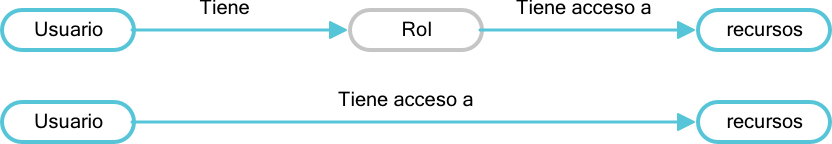
\includegraphics[width=1\textwidth]{firebase-auth}
  \caption{Autenticación basada en roles. (Fuente: Elaboración propia)}
\end{figure}

\subsubsection{Firebase Custom Claims}
Los roles de usuario son necesarios para identificar a los usuarios como administradores, gerentes o simplemente como clientes. Firebase Custom Claims permite establecer atributos de usuario simples directamente en el JWT del usuario (por ejemplo: \{ admin: true \}). Un JWT es un Json Web Token, es el objeto que contiene la información del usuario actual.
\vspace{0.8cm}

\lstinputlisting[label={firebase-auth}, style=ES6, caption=Fragmento para guardar crear y leer Firebase Custom Claims]{code/firebase-auth.js}

\subsection{Websockets con Socket.IO}
Si bien la base de datos Firebase Firestore proporciona una capa de conexión en tiempo real, es necesario introducir un nuevo método de comunicación permanente para notificar de eventos como lo son la presencia de usuarios activos y la visualización de las ordenes. Socket.IO permite la comunicación bidireccional entre el cliente y el servidor. Las comunicaciones bidireccionales se habilitan cuando un cliente tiene Socket.IO en el navegador, y un servidor también ha integrado el paquete. Si bien los datos se pueden enviar de varias formas, JSON es el más simple. Resume muchos tipos de transportes, incluidos \acrshort{ajax}  y \Glspl{websocket}, en una sola \acrshort{api}. Permite a los desarrolladores enviar y recibir datos sin preocuparse por la compatibilidad entre navegadores \cite{kelleher}.
\vspace{0.8cm}

En cualquier aplicación en tiempo real, mostrar múltiples usuarios en línea es muy importante, esta información debe actualizarse cuando un nuevo usuario se conecta o un usuario en línea se desconecta.
\vspace{0.8cm}

\begin{figure}[H]
  \centering
  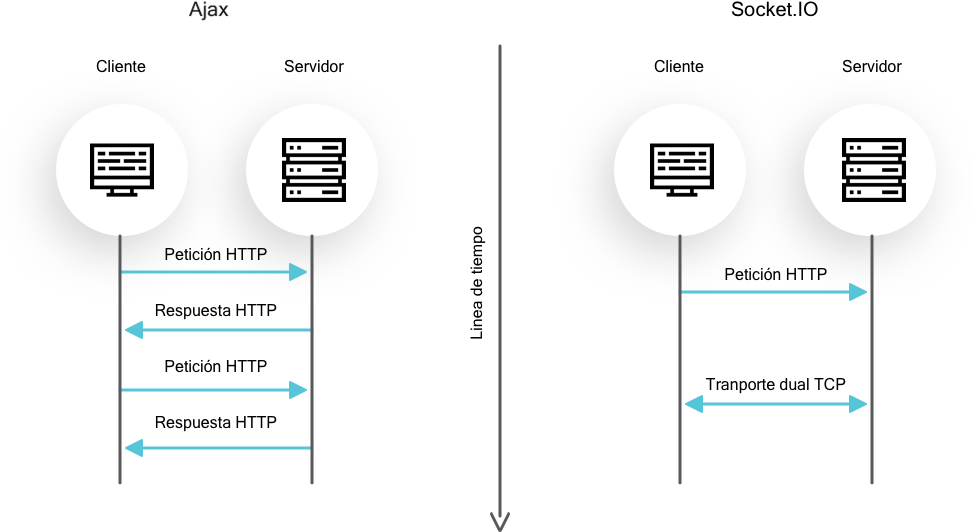
\includegraphics[width=1\textwidth]{websocket}
  \caption{Comparación de transporte por sondeo (Ajax) y Websockets (Socket.IO).}
\end{figure}

\lstinputlisting[style=ES6, caption=Fragmento de configuración de Socket.IO del sistema]{code/socket.js}


\newpage
\section{Desarrollo de la aplicación web (Frontend)}
El desarrollo de la aplicación web presenta grandes desafíos, debido a que en la actualidad existen un gran número de dispositivos móviles y navegadores web con características muy diferentes. Una buena aplicación web es más que algo para mirar, es funcional, interactiva e impecable. A medida que las tecnologías se vuelven inteligentes, debemos ser lo suficientemente inteligentes como para utilizarlas. Con la rápida evolución de las tecnologías web, la complejidad de las aplicaciones web también ha crecido, especialmente al hacer una aplicación web que funcione bien con todas las versiones de todos los navegadores \cite{ochin}.
\vspace{0.8cm}

El desarrollo web es un campo en constante cambio: la forma en que construimos sitios web hoy en día es completamente diferente de cómo solíamos hacerlo hace un par de años. Con la gran cantidad de herramientas disponibles y las nuevas que aparecen todos los días, la mayoría de las veces los desarrolladores se sienten confundidos sobre qué camino tomar.
\vspace{0.8cm}

\subsection{Configuración del entorno de desarrollo}
Los módulos en JavaScript, como en cualquier otro lenguaje de programación, ayudan a descomponer código en partes separadas más pequeñas. Este patrón ayuda a gestionar la creciente complejidad al mantener las preocupaciones separadas en sus partes independientes. En pocas palabras, los módulos ayudan a organizar el código.
\vspace{0.8cm}

Antes de ES6, esto se podía hacer usando diferentes archivos de \gls{script} y luego cargando cada uno de ellos por separado con una etiqueta \code{<script>} en nuestro HTML. Esto tenía muchas desventajas, como mantener el orden correcto de los \gls{script} para evitar romper accidentalmente cualquier código dependiente. Pero afortunadamente, ES6 trajo soporte para módulos con las palabras clave \code{import} y \code{export}, pero aún no son totalmente compatibles en todos los entornos (navegador y Node.js).
\vspace{0.8cm}

Webpack le permite escribir su código en módulos y unificarlos en uno o más paquetes. Webpack permite usar módulos y todas sus bondades sin preocuparse por el soporte. Además de JavaScript, también puede incluir otros tipos de archivos, incluidos (pero no limitados a) CSS, fuentes, imágenes, HTML, etc. y luego transformarlos en un formato aceptable. Webpack es extremadamente potente y se puede ampliar para hacer cosas impresionantes usando el concepto de loaders y \glspl{plugin}.
\vspace{0.8cm}

\subsubsection{Conceptos clave}
Webpack necesita una configuración básica para que funcione debidamente:

\begin{itemize}
  \item Entrada:
  Webpack utiliza el grafo de dependencias para decidir qué módulos deben agruparse. Esto significa que Webpack comienza desde un solo módulo y procesa todas sus dependencias directas e indirectas para formar el grafo de dependencia completo y luego agrupar todos los módulos necesarios.
  El punto de entrada determina desde dónde debe comenzar el paquete web para construir su gráfico de dependencia interna.\\
  Entrada del proyecto: \code{./src/app.js}
  \item Salida:
  La salida determina dónde se supone que el paquete web debe emitir los paquetes que crea y cómo los nombra. Este directorio también contendrá todos los archivos estáticos de la aplicación web que serán visibles al publico mediante el servidor Express.js.\\
  Salida del proyecto: \code{./www/bundle.js}
  \item Loaders
  Los loaders en el paquete web son los que le permiten manejar archivos que no son JavaScript (el empaquetador web solo comprende JavaScript). Los loaders leen varios tipos de archivos y los transforman en módulos válidos que webpack puede entender.
  \item Plugins
  Los \glspl{plugin} son la característica más poderosa de webpack, se utilizan para una amplia gama de tareas que los loaders no pueden realizar. Se utilizan  para la optimización de paquetes, \gls{minificacion}, emisión de estadísticas, etc.
\end{itemize}
\vspace{0.8cm}

\subsubsection{Babel Loader}
Babel ofrece el último soporte de sintaxis ECMAScript (ES5, ES6). Las librerías mas recientes insisten en que se utilicen las últimas ofertas de JavaScript para obtener un código más limpio y legible. Pero desafortunadamente nuestros navegadores no entienden la mayor parte de la sintaxis aquí es donde entra en juego Babel. Es responsable de convertir el código ES5 y ES6 en código comprensible por el navegador, básicamente compatibilidad con versiones anteriores. Las dependencias que necesita el proyecto son las siguientes:
\vspace{0.8cm}

\begin{itemize}
  \item babel-core: El motor principal de Babel para que sus dependientes trabajen.

  \item babel-preset-env: esta es la parte de soporte ES5, ES6

  \item babel-preset-react: Babel se puede usar en cualquier \gls{framework} que necesite el soporte de sintaxis JS más reciente, en este caso es `React'.

  \item babel-loader: Un puente de comunicación entre Webpack y Babel
\end{itemize}
\vspace{0.8cm}

\lstinputlisting[style=ES6, caption=Fragmeno de configuración Babel.]{code/babelrc.json}

\lstinputlisting[style=ES6, caption=Fragmeno de configuración Webpack]{code/webpack.js}

\subsubsection{Webpack Dev Server}
La herramienta Webpack Dev Server ejecuta y sirve una compilación de nuestro proyecto, pero no lo escribe en el disco, lo hace en la memoria. En modo de desarrollo, este modulo hace que la aplicación se abra un navegador, y vuelva a cargar el navegador cuando detecte cambios en los archivos de los que depende la aplicación web.
\vspace{0.8cm}

\lstinputlisting[style=ES6, caption=Configuración Webpack Dev Server.]{code/webpack.dev.js}

Con la ayuda de Webpack se tiene la capacidad de importar estilos y componentes de React y hacer que algo no solo sea funcional, sino también estético. Los procesos de construcción pueden ser desalentadores, pero si se tiene una base sólida y se sabe cómo expandirla, pueden obtenerse buenos resultados.
\vspace{0.8cm}

% \begin{figure}[H]
%   \centering
%   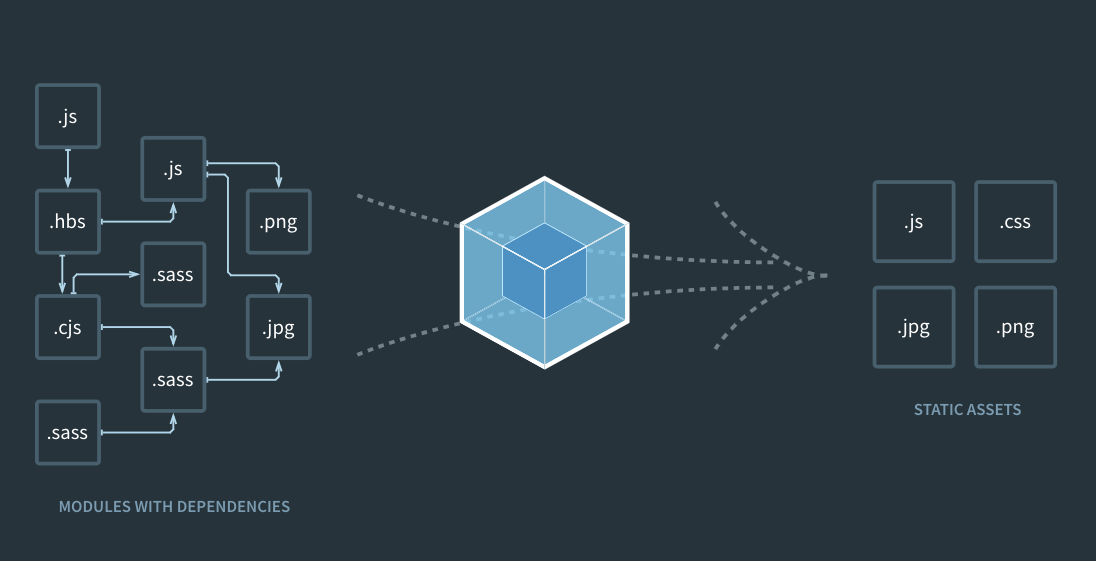
\includegraphics[width=1\textwidth]{webpack}
%   \caption{Imagen de la página oficial de Webpack donde se explica su concepto básico \cite{webpack}.}
% \end{figure}

\subsection{Patrones de diseño}
Las aplicaciones web modernas tienen una estructura de programa compleja, debido a las funcionalidades que proporcionan en sus interfaces de usuario. Escribir manualmente un código de programa puede dar como resultado una calidad y contenido desiguales en partes individuales de la aplicación. Mantener tales aplicaciones desarrolladas es más difícil. Debido a esto, las aplicaciones web a menudo se desarrollan utilizando diferentes \glspl{framework} y patrones de diseño.
\vspace{0.8cm}

Estos esquemas facilitan la reutilización de diseños y arquitecturas exitosas; también ayudan a elegir alternativas de diseño que hacen que un sistema sea reutilizable y evitar alternativas que comprometan la reutilización. Pueden incluso mejorar la documentación y el mantenimiento de los sistemas existentes.
\vspace{0.8cm}
Estos estándares de resolución de problemas pueden ser increíblemente útiles si se usan en las situaciones correctas y por las razones correctas. Cuando se usan estratégicamente, pueden hacer que un programador sea significativamente más eficiente al permitirle el usar métodos refinados por otros y evitar `reinventar la rueda'. También proporcionan un lenguaje común útil para conceptualizar problemas y soluciones repetidos cuando se discute con otros o se maneja el código en equipos más grandes.

\subsection{Redux}
Redux es un administrador de estado predecible para aplicaciones JavaScript basado en el patrón de diseño Flux. A medida que una aplicación crece, se hace difícil mantenerla organizada y mantener el flujo de datos. Redux resuelve este problema administrando el estado de la aplicación con un único objeto global llamado Redux Store. Los principios fundamentales de Redux ayudan a mantener la coherencia en toda la aplicación, lo que facilita la depuración y las pruebas. Redux se puede conectar con cualquier biblioteca de JavaScript. Sin embargo, funciona muy bien con ReactJS debido a su naturaleza funcional.
\vspace{0.8cm}

Redux ayuda a separar el estado de la aplicación, crea un almacén global que reside en el nivel superior de una aplicación y alimenta con el estado a todos los componentes internos. A diferencia de Flux, Redux no tiene múltiples objetos de almacenamiento. El estado completo de la aplicación está dentro de un objeto, y potencialmente podría intercambiar la capa de vista con otra biblioteca con el almacenamiento intacto.

\subsubsection{Redux/Flux}
Redux adoptó un gran número de restricciones de la arquitectura Flux: las acciones encapsulan la información para que el Redux Reducer actualice el estado de manera determinista, el estado es un Redux Store \gls{singleton}. El despachador de Flux único se reemplaza con múltiples Redux Reducers pequeños que recogen información de las acciones y la `reducen' a un nuevo estado que luego se guarda en el Redux Store. Cuando se cambia el estado en el Store, la Vista según la suscripción recibe propiedades llamadas props.
\vspace{0.8cm}

\begin{figure}[H]
  \centering
  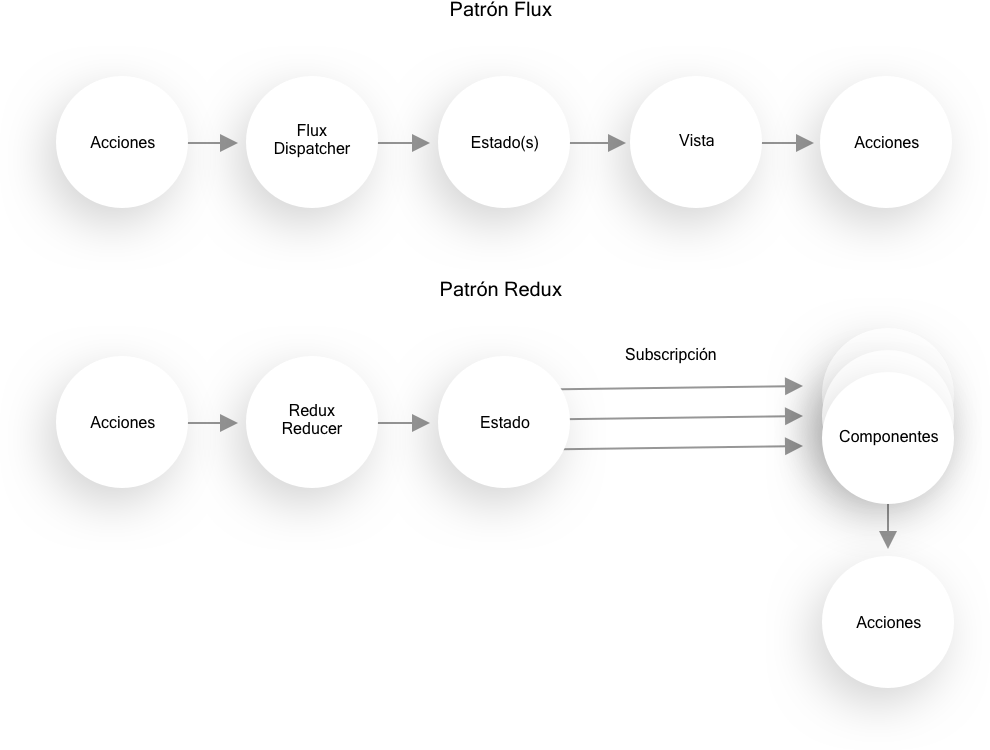
\includegraphics[width=0.9\textwidth]{flux-redux}
  \caption{Comparación Flux/Redux. (Fuente: Elaboración propia)}
\end{figure}
\vspace{0.8cm}

Para trabajar con Redux se necesitan tres cosas:
\begin{itemize}
  \item Actions (acciones): estos son objetos que deben tener dos propiedades, una que describe el tipo de acción y otra que describe lo que se debe cambiar en el estado de la aplicación.

  \item Reducers (reductores): son funciones que implementan el comportamiento de las acciones. Cambian el estado de la aplicación, en función de la descripción de la acción y la descripción del cambio de estado.

  \item Store (almacén): reúne las acciones y los reducers, manteniendo y cambiando el estado de toda la aplicación; solo hay una store.
\end{itemize}

\subsubsection{Redux Store}
Redux Store contiene un objeto del estado global de la aplicación. Esta actualiza el estado y notifica los componentes suscritos.
\vspace{0.8cm}

\lstinputlisting[style=ES6, caption=Fragmento de código para inicializar el Redux Store]{code/redux-store.js}

\subsubsection{Redux Reducer}
Un Redux Reducer es solo una función pura de JavaScript. Recibe dos parámetros: el estado actual y la acción. Una función pura es aquella que devuelve exactamente la misma salida para la entrada dada. El estado es el objeto Redux Store completo, la acción es el objeto despachado con un tipo requerido y un payload opcional.
\vspace{0.8cm}

\lstinputlisting[style=ES6, caption=Fragmento de código del reducer común de la app]{code/redux-reducer.js}

\subsubsection{Acciones Redux}
La única forma de cambiar el estado es enviando una señal al Store. Esta señal es una acción. Entonces "despachar una acción" significa enviar una señal a Redux Store.
\vspace{0.8cm}

\lstinputlisting[style=ES6, caption=Fragmento de una acción que actualiza el estado]{code/redux-action.js}

Este es un modelo conveniente y directo para estructurar datos en una aplicación y presentarlos en el cliente. La aplicación tiene un estado raíz. Un cambio de estado desencadena actualizaciones de vista. Solo las funciones especiales pueden modificar el estado. Una interacción del usuario activa estas funciones especiales de cambio de estado. Solo se produce un cambio a la vez. Esto significa que el estado central no puede desencadenar ninguna otra acción. Solo una entrada del usuario puede desencadenar otra acción \cite{mukhiya}.

\subsection{Integración React/Redux}
Redux practica la teoría de flujo de datos unidireccional y se convirtió en un patrón de facto como tecnología de gestión de estado para aplicaciones ReactJS. React utiliza \textit{props} (abreviatura de propiedades) en un componente que permite el uso de variables no estáticas. Con la ayuda de \textit{props}, podemos pasar estas variables a varios otros componentes (secundarios) desde el componente principal.
\vspace{0.8cm}

La conexión del Store de Redux con los componentes de React, es mediante un componente llamado \code{Provider} del módulo \code{react-redux}. En React para compartir datos entre componentes, un estado tiene que vivir en el componente principal. Este componente principal proporciona un método para actualizar este estado y se pasa como \textit{props} a estos componentes. El único propósito de \code{Provider} es agregar el Store al contexto del componente de la Aplicación, para que todos los componentes secundarios puedan acceder a ella mediante la función \code{connect} de \code{react-redux}. \code{Provider} envuelve a la aplicación React y hace que sea consciente de el Store.
\vspace{0.8cm}

\lstinputlisting[style=ES6, caption=Fragmento de código de la aplicación React principal]{code/redux-react.js}

La función \code{connect} ayuda a conectar un componente con el estado de la aplicación, se debe definir una función especial llamada \code{mapStateToProps} para describir que partes del estado actual de Redux se desean pasar al componente que está envolviendo y una función de nombre \code{mapDispatchToProps} conecta las acciones de Redux con React \textit{props}. De esta manera, un componente React conectado podrá enviar mensajes a el Store.
\vspace{0.8cm}

\lstinputlisting[style=ES6, caption=Ejemplo de conexión de un componente React con el estado Redux]{code/connect.js}
% \begin{enumerate}
%   \item El primer argumento es
% \end{enumerate}

\subsection{Diseño Atómico (Atomic Design)}
El diseño atómico es una metodología compuesta por cinco etapas distintas que trabajan juntas para crear sistemas de diseño de interfaz de una manera más deliberada y jerárquica. Las cinco etapas del diseño atómico son:
\vspace{0.8cm}

\begin{enumerate}
  \item Átomos
  \item Moléculas
  \item Organismos
  \item Plantillas
  \item Páginas
\end{enumerate}
\vspace{0.8cm}

El diseño atómico no es un proceso lineal, sino un modelo mental que nos ayuda a pensar en nuestras interfaces de usuario como un todo cohesivo y una colección de partes al mismo tiempo. Cada una de las cinco etapas juega un papel clave en la jerarquía de nuestros sistemas de diseño de interfaz \cite{frost}.
\vspace{0.8cm}


\begin{figure}[H]
  \centering
  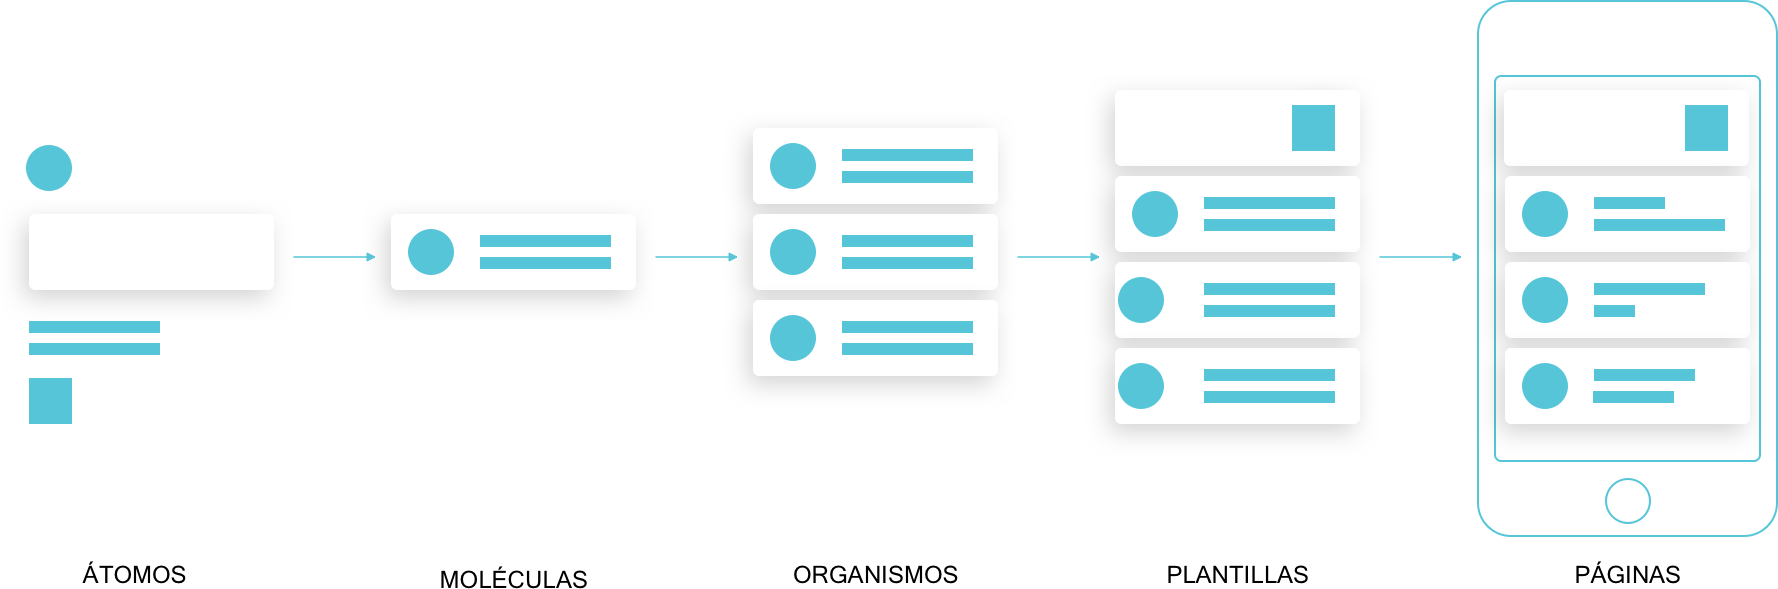
\includegraphics[width=1\textwidth]{atomic}
  \caption{Metodología de diseño atómico. (Fuente: Elaboración Brad Frost 2016)}
\end{figure}

\subsection{Estructura de la aplicación web}
La interfaz de usuario juega un papel muy importante en el aumento de la usabilidad de una aplicación, dado que la IU ofrece al usuario una vista abstracta de todo el sistema, el éxito del sistema depende en gran medida de ello. Por lo tanto, el diseño de la interfaz de usuario debe tener la importancia adecuada en el proceso del ciclo de vida del diseño del sistema.
\vspace{0.8cm}

\subsubsection{Módulo de inicio de sesión}
Uno de los desafíos es cómo implementar un esquema de autenticación y autorización flexible, seguro y eficiente. Parece confuso diferenciar entre autenticación y autorización. De hecho, es muy simple.

\begin{itemize}
  \item Autenticación: se refiere a verificar `quién es usted', por lo que debe usar el nombre de usuario y la contraseña para la autenticación.

  \item Autorización: se refiere a lo que `puede hacer', por ejemplo, acceder, editar o eliminar datos a algunos documentos, esto sucede después de la verificación.
\end{itemize}

Firebase Authentication proporciona servicios de back-end, SDK fáciles de usar y bibliotecas de interfaz de usuario para autenticar a los usuarios en la aplicación. En el código ejemplo \ref{login} se muestran los métodos necesarios para el manejo de sesiones del proyecto.
\vspace{0.8cm}

\lstinputlisting[style=ES6, label=login, caption=Fragmento de código del manejo de sesión de usuario]{code/login.js}

Gracias a la simplicidad y efectividad de los servicios de Firebase, este proceso es utilizado por muchas aplicaciones y servicios web en la actualidad.
\vspace{0.8cm}

\subsubsection{Evaluación de la interfaz de usuario}
El objetivo del proyecto es señalar los problemas y desafíos que surgen del uso de una pantalla táctil como dispositivo de entrada en una aplicación web. Para lograr esto, se desarrolló un prototipo, basado en pautas teóricas. El prototipo fue evaluado en sesiones informales donde los usuarios lo probaron y hablaron sobre cómo lo percibieron. Se alentó a los sujetos a sugerir soluciones alternativas y criticar las soluciones que encontraron negativas.
\vspace{0.8cm}

El prototipo inicial sufrió muy pocos cambios, siendo principalmente por motivos de funcionalidad y no estéticos. Todos los usuarios que sometieron a prueba la aplicación acordaron que el diseño era fácil de entender y se podían acostumbrar a el rápidamente. El resultado de la evaluación demostró que la interfaz responsiva funciona adecuadamente.

\newpage
\section{Configuración para producción}
Hacer que las aplicaciones de Node.js estén listas para producción es probablemente el tema más oculto y omitido en la literatura de Node.js, pero es uno de los más importantes \cite{mardan}. Se requiere de un método estandarizado para que la efectividad del despliegue en el servidor de producción sea optima.

\subsubsection{Requisitos del servidor}

\begin{itemize}
  \item Servidor CentOS 7 con Node.js y Git instalado.
  \item Al menos 512 Mb de RAM y 15 Gb de espacio libre en disco.
  \item Acceso de usuario root a través de SSH.
  \item Un nombre de dominio apuntado a la dirección IP del servidor (caminapp.app)
  % \item Editor de texto nano, puede instalarse con este comando:\\
  
  % \code{yum install nano}
\end{itemize}

\subsubsection{Servidor Privado Virtual}
Esta tecnología permite ejecutar las instancias de múltiples servidores en un servidor host físico de forma segura. Es un tipo de servidor de alojamiento web donde el alojamiento generalmente se realiza dividiendo un servidor físico principal en diferentes servidores virtuales múltiples. Cada uno de los servidores del sistema obtiene su propia parte de los recursos en función de los requisitos del cliente.
\vspace{0.8cm}

Este proyecto utiliza un servidor privado virtual (VPS) alojado en Digital Ocean, en donde debe decidir qué sistema operativo se desea, configurar el acceso SSH, crear un firewall, instalar los distintos lenguajes que necesita, etcétera. Para crear el VPS para el proyecto se accede a www.digitalocean.com y se crea una cuenta en Digital Ocean. Es necesario verificar la cuenta con una dirección de correo electrónico antes de poder crear un proyecto. Una vez verificada la dirección de correo electrónico, deberá un método de pago para el servicio. Al finalizar el registro y el modo de financiamiento se puede comenzar a configurar un servidor o Droplet. En Digital Ocean un Droplet es una máquina virtual simple y escalable. Con un costo de solo 5 dolares al mes, el plan básico es lo suficiente para mantener el proyecto en operación.
\vspace{0.8cm}

\begin{figure}[H]
  \centering
  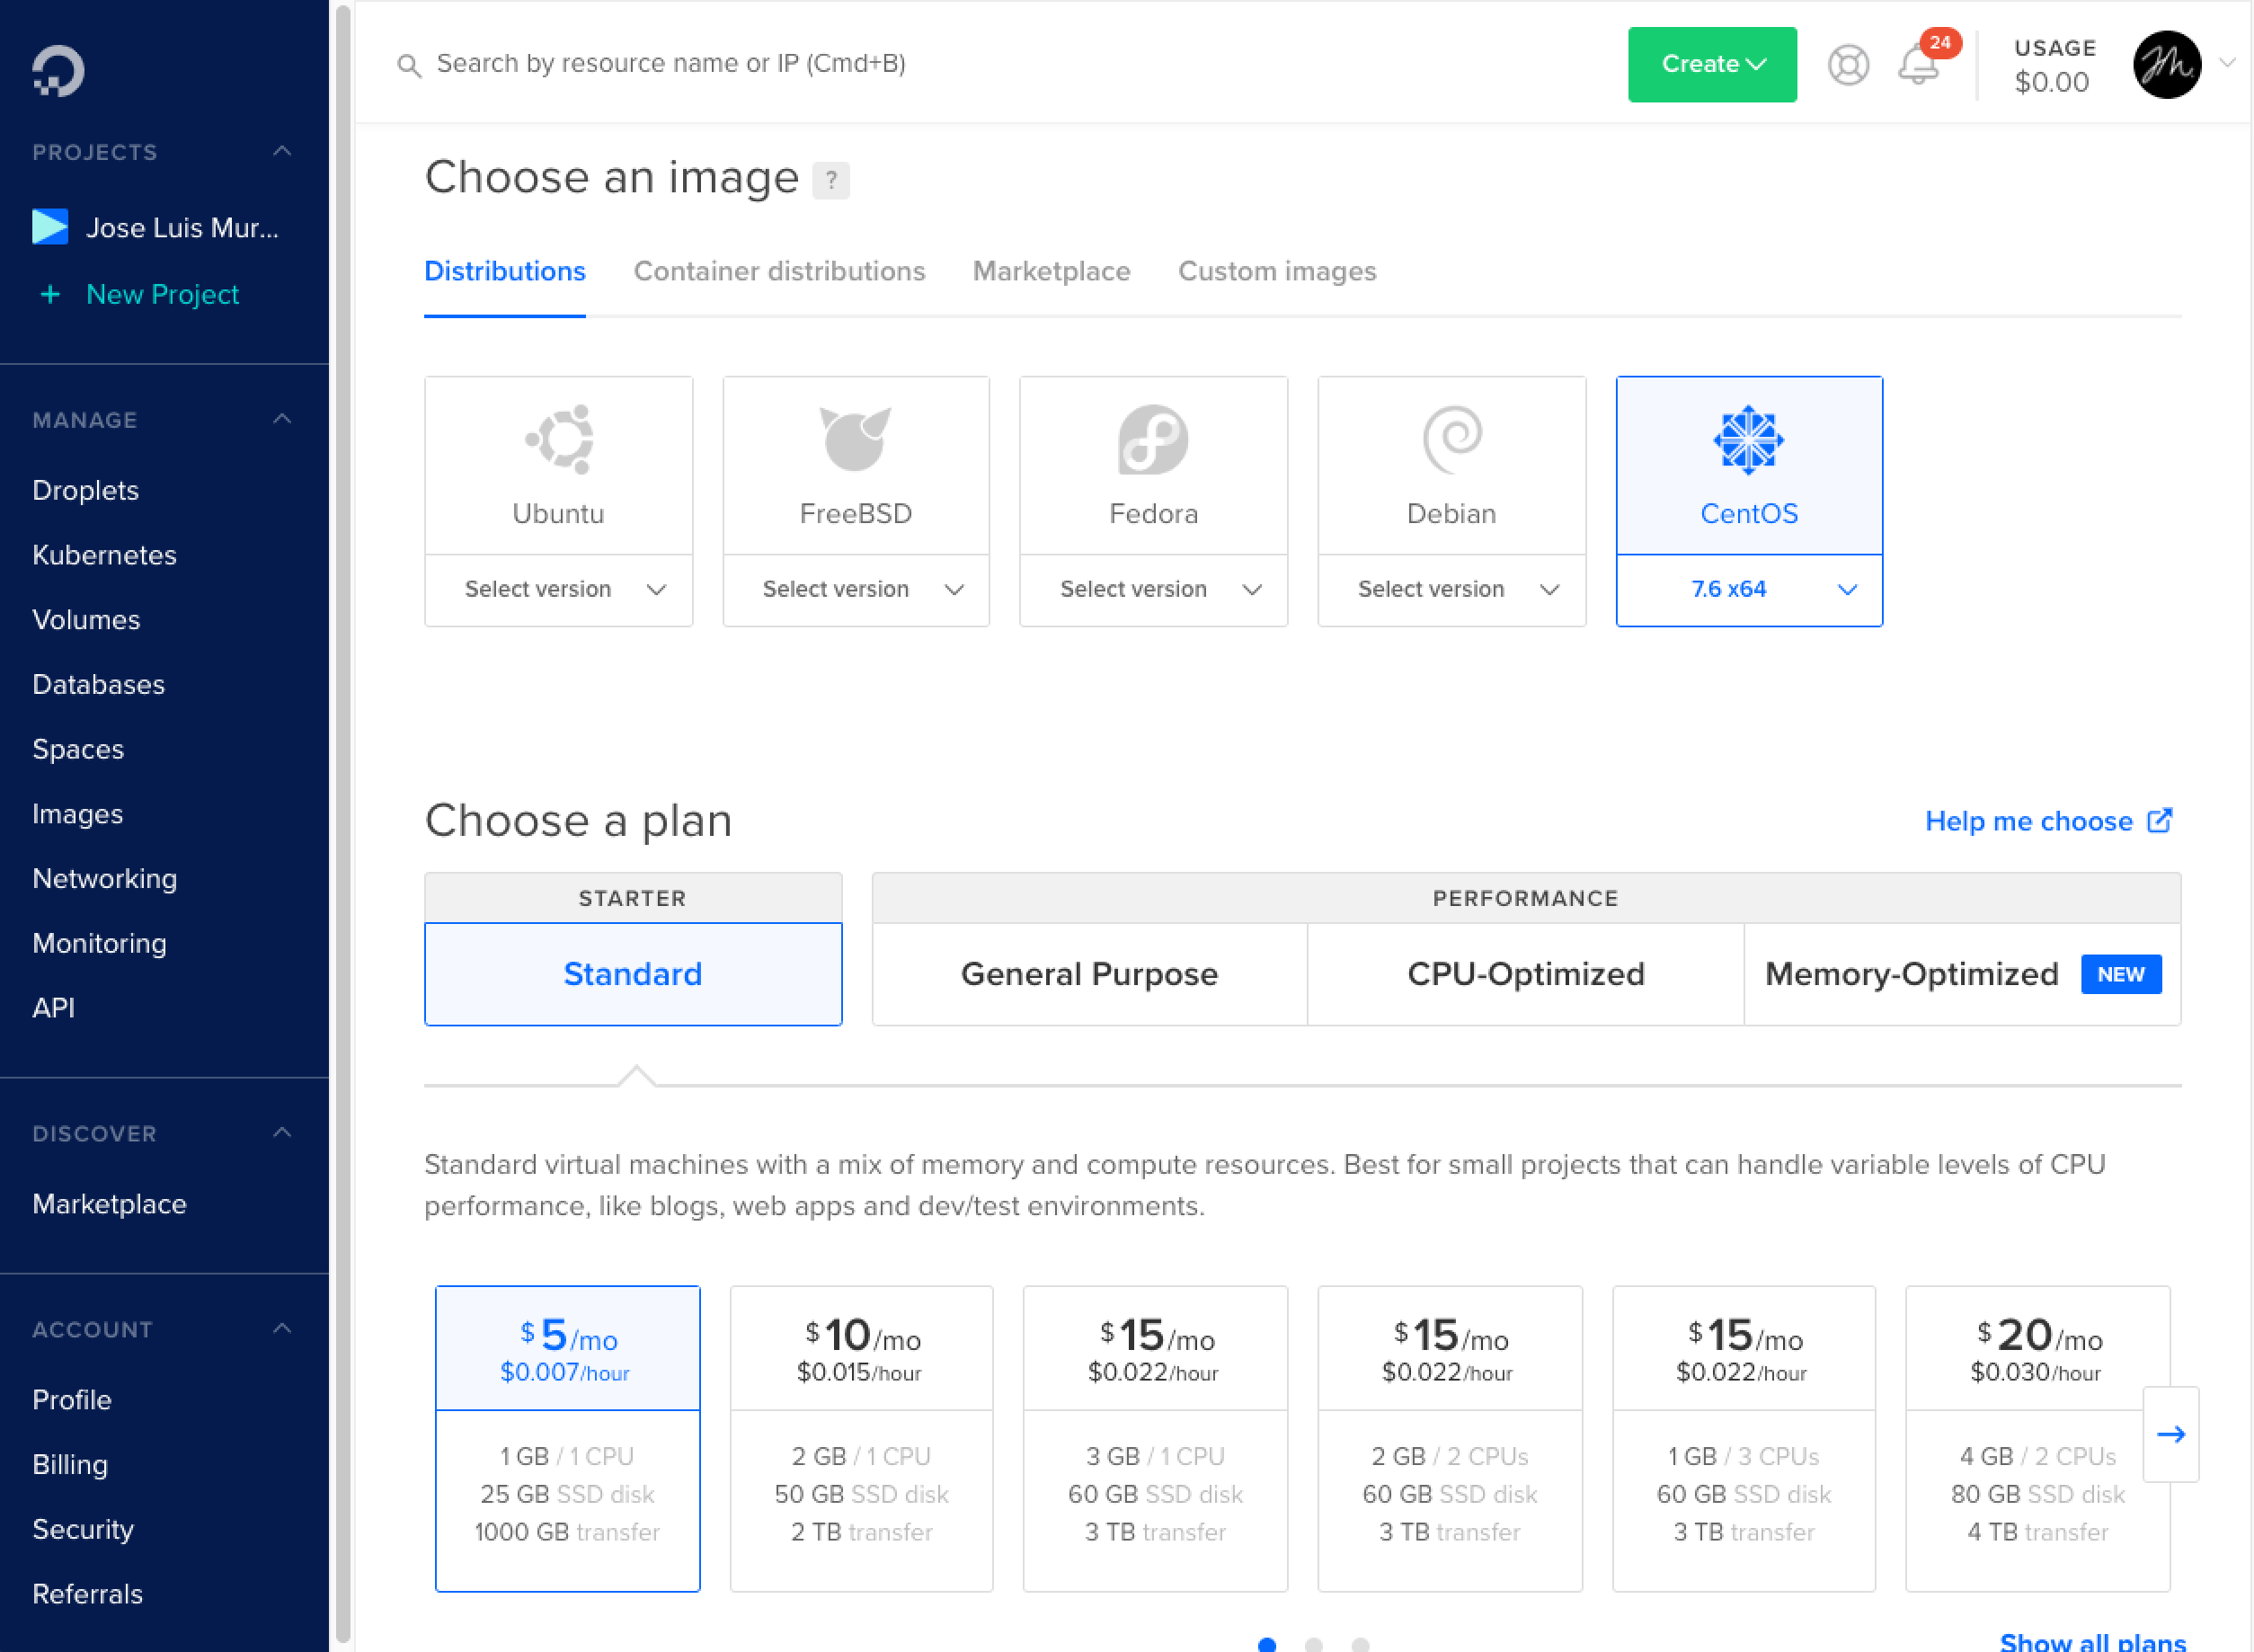
\includegraphics[width=1\textwidth]{digital-ocean}
  \caption{Configuración básica del servidor virtual privado. (Fuente: Digital Ocean)}
  \label{digital-ocean}
\end{figure}

Una vez que el servidor es creado, se recibe un correo electrónico de Digital Ocean. Este correo electrónico contiene los detalles de inicio de sesión para el servidor, en donde podremos conectarnos mediante SSH.
\vspace{0.8cm}

\subsection{Configurar despliegue automático con Git}
Al utilizar Git, el flujo de trabajo generalmente se dirige solo al control de versiones. Se tiene un repositorio local donde se trabaja y un repositorio remoto donde se mantiene todo sincronizado y se puede trabajar con un equipo y diferentes máquinas. Pero también es posible usar Git para mover una aplicación a producción \cite{vaccaro}.
\vspace{0.8cm}

\subsubsection{Configuración de repositorios}
Para poder empujar cambios a nuestro repositorio remoto se debe establecer la siguiente estructura:

\begin{itemize}
  \item Directorio publico del servidor: /var/www/caminapp.app
  \item Directorio del repositorio del servidor: /var/repo/site.git
\end{itemize}

Se inicia sesión en el VPS desde la consola de comandos y se ingresa lo siguiente:\\
\\
\code{cd /var}\\
\code{mkdir repo \&\& cd repo}\\
\code{mkdir site.git \&\& cd site.git}\\
\code{git init ---bare}\\

\code{---bare} significa que la carpeta no tendrá archivos fuente, solo el control de versiones.

\subsubsection{Git Hooks}
Los repositorios de Git tienen una carpeta llamada \code{hooks}. Esta carpeta contiene algunos archivos de muestra para conectar y realizar acciones personalizadas. La documentación de Git define tres posibles enlaces de servidor: \textit{pre-recepción}, \textit{post-recepción} y \textit{actualización}. Para este proyecto se necesita un `\gls{hook}' para post-recepción, que se ejecuta cuando un `envío' está completamente terminado.
\vspace{0.8cm}

En el repositorio se encuentran algunos archivos y carpetas, incluida la carpeta \code{hooks}. Se accede a ella mediante el siguiente comando.\\
\\
\code{cd hooks}\\
\\
Se crea el archivo post-recepción escribiendo:\\
\\
\code{cat > post-receive}\\
\\
Al ejecutar este comando, se muestra una línea en blanco que indica que todo lo que escriba se guardará en este archivo. Se debe agregar lo siguiente:\\
\\
\code{\#!/bin/sh}\\
\code{git --work-tree=/var/www/caminapp.app --git-dir=/var/repo/site.git checkout -f}\\
\\
Al terminar, se presiona `control-d' para guardar. Para ejecutar el archivo, se necesita establecer los permisos adecuados usando:\\
\\
\code{chmod +x post-receive}\\
\\
El archivo post-recepción se examina cada vez que se completa un envío y coloca los archivos en \code{/var/www/caminapp.app}, esto permite actualizaciones directas del proyecto facilitando el mantenimiento de codigo y evitando la tarea de tener que conectarse al servidor para cargar los archivos manualmente.
\vspace{0.8cm}

En el repositorio local se necesita configurar la ruta del repositorio remoto. Se le dice Git que agregue un control remoto llamado `live':\\
\\
\code{git remote add live ssh://root@caminapp.app/var/repo/site.git}\\
\\
Con esto es posible empujar cambios en el repositorio al servidor remoto usando el alias `live':\\
\\
\code{git push live master}\\
\\
Con esto se le dice a Git que empuje al remoto `live' en la rama `master'.
\vspace{0.8cm}

\subsection{Despliegue Node.js en un entorno de producción}
El término servidor puede ser un poco confuso para las personas nuevas en el tema porque puede referirse tanto al \gls{hardware} (computadoras físicas que albergan todos los archivos requeridos por los sitios web) como al \gls{software} (programa que permite a los usuarios acceder a esos archivos en la web). El \gls{hardware} se encuentra alojado en un servidor virtual privado, por tal motivo esta sección se centra en el lado del software.

\subsubsection{Servidor proxy inverso}
Una vez transferido el código del proyecto al servidor y configurar un entorno para la aplicación, es momento de configurar un servidor proxy inverso. Un servidor proxy es un servidor intermedio o intermediario que reenvía solicitudes de contenido de varios clientes a diferentes servidores a través de Internet. Un servidor proxy inverso es un tipo de servidor proxy que generalmente se encuentra detrás del firewall en una red privada y dirige las solicitudes de los clientes al servidor apropiado. Un proxy inverso proporciona un nivel adicional de abstracción y control para garantizar el flujo fluido del tráfico de red entre clientes y servidores.

\subsubsection{Configuración nginx y firewall-cmd}
Nginx (Engine X) es una de las mejores soluciones para configurar un servidor proxy inverso, con el será posible entregar contenido de forma rápida, confiable y segura. Hará que la aplicación sea accesible desde un navegador, y en caso de ejecutar varios sitios desde el mismo servidor, también podría funcionar como equilibrador de carga.
\vspace{0.8cm}

Después de iniciar sesión como usuario root, se agrega el repositorio CentOS 7 \acrshort{epel} y se instala nginx con los siguientes comandos:\\
\\
\code{yum install epel-release}\\
\code{yum install nginx}\\
\\
Se presiona ‘y’ dos veces para finalizar la instalación. Para inicializar el servicio nginx y este inicie con el arranque del servidor se introducen los siguientes comandos:\\
\\
\code{sudo systemctl enable nginx}\\
\code{sudo systemctl start nginx}\\
\\
A continuación se instala firewall-cmd, el front-end de línea de comandos para firewalld (\gls{daemon} firewalld), para CentOS. Admite IPv4 e IPv6, zonas de firewall, puentes y conjuntos de ip, registra paquetes denegados, carga automáticamente módulos de \gls{kernel}, entre otras cosas más. Se instala con el siguiente comando:\\
\\
\code{yum install firewalld}\\
\\
Ahora, se habilita para que se inicie automáticamente en el arranque del sistema y se observa su estado:\\
\\
\code{systemctl start firewalld}\\
\code{systemctl enable firewalld}\\
\code{systemctl status firewalld}\\
\\
En nginx para CentOS se necesita crear carpetas para sitios disponibles y habilitados. Se crean con los siguientes comandos:\\
\\
\code{mkdir /etc/nginx/sites-available}\\
\code{mkdir /etc/nginx/sites-enabled}\\
\\
Después se edita el archivo de configuración global de nginx:\\
\\
\code{nano /etc/nginx/nginx.conf}\\
\\
Se identifica la linea:\\
\\
\code{include /etc/nginx/conf.d/*.conf;}\\
\\
Se inserta lo siguiente:\\
\\
\code{include /etc/nginx/sites-enabled/*;}\\
\code{server\_names\_hash\_bucket\_size 64;}
\vspace{0.8cm}

\begin{lstlisting}[language=bash, caption=Fragmento de configuración nginx]
http {
  include       /etc/nginx/mime.types;
  default_type  application/octet-stream;

  log_format  main  '$remote_addr - $remote_user [$time_local] "$request" '
                    '$status $body_bytes_sent "$http_referer" '
                    '"$http_user_agent" "$http_x_forwarded_for"';
  access_log  /var/log/nginx/access.log  main;
  sendfile        on;
  keepalive_timeout  65;

  #Se agrega debajo de esta linea
  include /etc/nginx/conf.d/*.conf;
  include /etc/nginx/sites-enabled/*;
  server_names_hash_bucket_size 64;
}
\end{lstlisting}

Para finalizar se procede a utilizar el modulo npm llamado `nginx-generator' para generar los archivos que le indican a nginx que actúe como un proxy inverso. En la linea de comandos se escribe lo siguiente:\\
\\
\code{nginx-generator \symbol{92}}\\
\code{        ---name caminapp \symbol{92}}\\
\code{        ---domain http://caminapp.app \symbol{92}}\\
\code{        ---type proxy \symbol{92}}\\
\code{        ---var host=localhost \symbol{92}}\\
\code{        ---var port=3000 \symbol{92}}\\
\code{        /etc/nginx/sites-enabled/caminapp.app.conf}\\
\\
Este comando crea un archivo llamado \code{site\_nginx} y lo coloca dentro del directorio \code{/etc/nginx/sites-enabled/}. El archivo se puede observar con el siguiente comando:\\
\\
\code{sudo nano /etc/nginx/sites-enabled/caminapp.app.conf}\\
\\
Por ultimo se reinicia nginx:\\
\\
\code{systemctl restart nginx}

\subsubsection{Configuración del administrador de procesos PM2}
PM2 es un administrador de procesos de producción para aplicaciones basadas en Node.js. Con PM2, se pueden monitorear aplicaciones, su memoria y uso de CPU. También proporciona comandos fáciles para detener/iniciar/reiniciar todas las aplicaciones o aplicaciones individuales. Una vez que la aplicación se inicia a través de PM2, siempre se ejecutará después de que el sistema se bloquee o reinicie.
\vspace{0.8cm}

PM2 se instala mediante npm con el siguiente comando:\\
\\
\code{npm install pm2 -g}\\
\\
Una vez instalado sera posible ejecutar la aplicación con PM2:\\
\\
\code{pm2 start /var/www/caminapp.app/index.js ---name caminapp}\\

\begin{figure}[H]
  \centering
  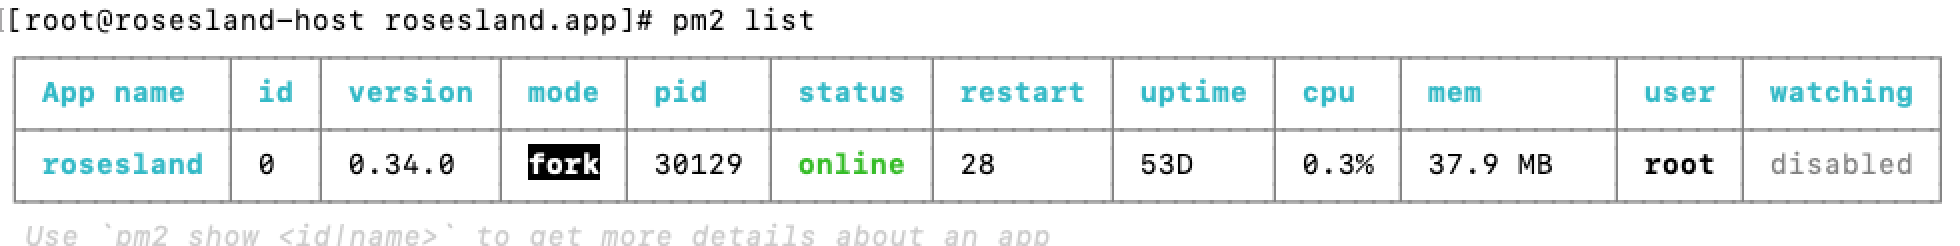
\includegraphics[width=1\textwidth]{pm2}
  \caption{Lista de procesos en pm2. (Fuente: Elaboración propia)}
\end{figure}

\subsubsection{Asegurar el sitio mediante HTTPS}
Con un nombre de dominio y registros DNS configurados correctamente para que apunten al VPS, se puede usar Certbot para generar certificados. Certbot es una herramienta de software gratuita y de código abierto para usar automáticamente certificados seguros en sitios web administrados manualmente para habilitar HTTPS \cite{certbot}.
\vspace{0.8cm}

Certbot está empaquetado en los Paquetes Adicionales para Enterprise Linux o EPEL (Extra Packages for Enterprise Linux). Para habilitar el repositorio adicional, el canal opcional e instalar EPEL, se emiten los siguientes comandos:\\
\\
\code{yum -y install yum-utils}\\
\code{yum-config-manager --enable \symbol{92}}\\
\code{rhui-REGION-rhel-server-extras rhui-REGION-rhel-server-optional}\\
\code{sudo yum install certbot python2-certbot-nginx}\\
\\
Se presiona `y' cuando es requerido y al finalizar ejecutamos certbot:\\
\\
\code{certbot --nginx}\\
\\
Cuando se instalan certificados por primera vez, Certbot pide una dirección de correo electrónico de emergencia, luego varias preguntas menos importantes y, finalmente, ¿desea redirigir todo el tráfico HTTP a HTTPS? Se selecciona la opción 2 para confirmar esta redirección y concluir con la configuración del despliegue de la aplicación.
\vspace{0.8cm}

En este momento se cuenta con una aplicación Node.js ejecutándose como un servicio en segundo plano en un entorno de producción, utilizando el protocolo HTTPS por seguridad y nginx como proxy inverso.


\subsubsection{Apache Cordova}
Apache Cordova es un marco de desarrollo móvil de código abierto. Le permite utilizar tecnologías web estándar: HTML5, CSS3 y JavaScript para el desarrollo multiplataforma. Las aplicaciones se ejecutan dentro de contenedores dirigidos a cada plataforma, y se basan en enlaces API que cumplen con los estándares para acceder a las capacidades de cada dispositivo, como sensores, datos, estado de la red, etc. Sus principales funciones engloban \ref{cordova}:

\begin{enumerate}
  \item Extender una aplicación en más de una plataforma, sin tener que volver a implementarla con el conjunto de herramientas y lenguaje de cada plataforma.
  \item Implementar una aplicación web que está empaquetada para su distribución en varios portales de la tienda de aplicaciones.
  \item Mezclar componentes de aplicaciones nativas con un WebView (ventana de navegador especial) que puede acceder a las API a nivel de dispositivo, o si desea desarrollar una interfaz de complemento entre los componentes nativos y WebView.
\end{enumerate}

\subsubsection{Crear una aplicación Cordova}
La herramienta de línea de comandos Cordova se distribuye como un paquete npm. Para instalar la herramienta de línea de comandos cordova, se siguen estos pasos:

\begin{enumerate}
  \item Descargar e instalar Node.js. En la instalación, debería poder invocar node y npm en la línea de comando.
  \item (Opcional) Descargar e instalar un cliente git, si aún no tiene uno. Después de la instalación, se debería poder invocar git en la línea de comando. La CLI se usa para descargar activos cuando se hace referencia a ellos utilizando una url a un repositorio git.
  \item Instalar el módulo cordova usando la utilidad npm de Node.js. La utilidad npm descargará automáticamente el módulo cordova.
\end{enumerate}

En OS X y Linux:

\code{sudo npm install -g cordova}\\

En OS X y Linux, puede ser necesario agregar el comando \code{npm} con \code{sudo} para instalar esta utilidad de desarrollo en directorios restringidos como \code{/usr/local/share}. Si se utiliza la herramienta opcional \code{nvm} o se tiene acceso de escritura al directorio de instalación, se puede omitir el prefijo sudo.


En Windows:

\code{npm install -g cordova}
El indicador \code{-g} anterior le dice a npm que instale cordova a nivel global. De lo contrario, se instalará en el subdirectorio node_modules del directorio de trabajo actual.

\subsubsection{Crear la aplicación}
En el folder donde se mantendrá el proyecto se ejecuta el siguiente comando:

\code{cordova create caminapp com.example.caminapp Caminapp}

Esto crea la estructura de directorios requerida para la aplicación cordova. Por defecto, el script de creación cordova genera una aplicación esquelética basada en la web cuya página de inicio es el archivo \code{www/index.html} del proyecto.

\subsubsection{Agregar plataformas}
Todos los comandos posteriores deben ejecutarse dentro del directorio del proyecto o en cualquier subdirectorio:

\code{cd caminapp}

Se agregan las plataformas a las que desea orientar la aplicación. Agregaremos la plataforma 'ios' y 'android' y nos aseguraremos de que se guarden en \code{config.xml} y \code{package.json}

\code{cordova platform add ios}
\code{cordova platform add android}

\subsubsection{Instalar requisitos previos para construir}
Para compilar y ejecutar aplicaciones, se deben instalar SDK para cada plataforma a la que desee apuntar. Alternativamente, si se está usando el navegador para el desarrollo, puede usar la plataforma del navegador que no requiere ningún SDK de plataforma.

Para verificar si cumple con los requisitos para construir la plataforma:

\code{cordova requirements}

\subsubsection{Compilar}
Ejecute el siguiente comando para generar el proyecto para todas las plataformas:
\code{cordova build}
Opcionalmente, se puede limitar el alcance de cada compilación a plataformas específicas: 'ios' en este caso:
\code{cordova build ios}


\subsubsection{Agregar Plugins}
Se puede modificar la aplicación generada por defecto para aprovechar las tecnologías web estándar, pero para que la aplicación acceda a las funciones a nivel de dispositivo, deben agregar complementos.

Un complemento expone una API de Javascript para la funcionalidad nativa del SDK. Los complementos generalmente se alojan en npm y puede buscarlos en la página de búsqueda de complementos. Algunas API clave son proporcionadas por el proyecto de código abierto Apache Cordova y se denominan API Core Plugin. Por ejemplo, para agregar y guardar el complemento de la cámara en config.xml y package.json, especificaremos el nombre del paquete npm para el complemento de la cámara:

\code{cordova plugin add cordova-plugin-camera}

\chapter{Conclusiones}
Los procedimientos establecidos al crear este proyecto sirven como base para elaborar otras aplicaciones, su código es escalable y permite integrar un gran numero de servicios y \glspl{framework}, por lo que su limitación solo estará marcada por las necesidades de los usuarios.
\vspace{0.8cm}



\printbibliography

\printglossary

\clearpage

\printglossary[type=\acronymtype]

\end{document}